%%%%%%%%%%%%%%%%%%%%%%%%%%%%%%%%%%%%%%%%%%%%%%%%%%%%%%%%%%%%%%%%%%%%%%%%%%%%%%%
%%% Modèle de thèse électronique pour les sciences (c) Jean Hare 2017
%%%%%%%%%%%%%%%%%%%%%%%%%%%%%%%%%%%%%%%%%%%%%%%%%%%%%%%%%%%%%%%%%%%%%%%%%%%%%%%
%%% Format personnalisé avec %& :  doit figurer  seul sur la 1ière ligne %
%%&"mythesis"
%%% Les trois commentaires spéciaux ci-dessous sont destinés à l'éditeur TeXWorks
% !TeX encoding = UTF-8
% !TeX program = pdflatex 
% !TeX spellcheck = fr_FR
\documentclass[a4paper,11pt]{book} %ADD diffusion OR archiv for final versions
\usepackage[utf8]{inputenc}
%\usepackage[latin9]{inputenc}
\usepackage{xspace}			  
\usepackage[english]{babel}
\usepackage[T1]{fontenc}
\usepackage{lmodern}
\usepackage[margin=28mm,includeheadfoot,bindingoffset=5mm]{geometry}
\usepackage{thcover}
\usepackage{physics}
% !TeX encoding = UTF-8
%%% préamble pour les graphiques %%%
\usepackage{graphicx,color} 
\usepackage[svgnames]{xcolor} %seuls les noms des couleurs sont pris dans SVG
%%% pour des graphiques incrustés dans le texte, déconseillé pour une thèse,
%\usepackage{wrapfig,picins} %  %éviter wrapfig et picins au profit de floatflt
%\usepackage{floatflt}
%%% Pour un meilleur contrôle des objets flottants (figures, tables)
\renewcommand{\topfraction}{0.7}     % autorise 70% page de graphique en haut
\renewcommand{\bottomfraction}{0.5}  % autorise 50% page de graphique en bas
\renewcommand{\floatpagefraction}{0.7}
\renewcommand{\textfraction}{0.1}
%%% Format français des légendes
\usepackage{subcaption}
\captionsetup[figure]{name=Fig.,labelsep=quad,labelfont=normalfont,textfont=sl,%
   singlelinecheck=true,width=0.9\linewidth}
%%% Autres paquets
%\usepackage{placeins}   % pour  \FloatBarrier
%\usepackage{epstopdf}   % pour inclure des eps
%\usepackage{pdfpages}   % por inclure de portions d fichiers PDF
%\usepackage{float} \usepackage{nonfloat} \usepackage{endfloat} \usepackage{topfloat}
%%% Chemin des figures
%\graphicspath{{./fig1/},{../fig2/}}
\usepackage{svg}

% !TeX encoding = UTF-8
%%% préamble pour les maths %%%

\usepackage{amsmath}

%\usepackage{amsmath, mathtools}
%\mathtoolsset{showonlyrefs}
\usepackage{amsfonts,bm,bbm}     % mathématique de AMS + boldmathth et blackboard
\usepackage{upgreek}             % lettres grecques pour μm et pour β-decay


%\usepackage{mathdots}           % points pour matrices et dérivées
%\usepackage{icomma}             % virgule séparateur numérique%\mathtoolsset{showonlyrefs,showmanualtags}
%\usepackage[overload]{abraces}  % des accolades horizontales plus élégantes
%\usepackage[e]{esvect}          % des flèches de vecteurs plus élégantes
%\usepackage{esint}		      % intégrales diverses; installer esint-type1
%\usepackage{pifont}             % zapfdingbats; do you _really_ need them ?
%\DeclareUnicodeCharacter{03C3}{\sigma}       % σ  (disponible seulement en utf8)

% !TeX encoding = UTF-8
%%% préamble pour les utilitaires %%%
\usepackage{etoolbox}          % nombreuses fonctions avancées
\usepackage{calc}              % calcul infix des longueurs
\usepackage{datetime}                % fonctions d'heure et de temps
\usepackage{eso-pic}                 % pour placer des éléments en fond de page


% !TeX encoding = UTF-8
%%% préamble pour les titres et entêtes %%%
%%% TikZ % à completer avecles \usetkzlibrary{} nécessaires
%\usepackage{tikz}
%\usepgfmodule{decorations}
%\usetikzlibrary{calc,patterns,spy,decorations,arrows,matrix,positioning,decorations.pathreplacing, decorations.pathmorphing}
%\BeforeBeginEnvironment{tikzpicture}{\shorthandoff{:;!?}}
%\AfterEndEnvironment{tikzpicture}{\shorthandon{:;!?}}
%%% Entêtes : l'option "headings" est  normalement suffisante
%%% Pour passer localement à "myheadings" : \thispagestyle{myheadings} \markboth{<left>}{<right>}
\pagestyle{headings}
\usepackage{slantsc}
\makeatletter
\patchcmd{\chaptermark}{\MakeUppercase}{\scshape\slshape}{}{}%
\patchcmd{\sectionmark}{\MakeUppercase}{\scshape\slshape}{}{}%
\patchcmd{\sectionmark}{\thesection.}{\thesection}{}{}       % suppression du point IV.1. -> IV.1
\makeatother
%%% Réglages des numérotations
\setcounter{secnumdepth}{4}                          % numérote chapter, section, sub(sub)sect
\setcounter{tocdepth}{3}                             % profondeur de la table des matieres
\numberwithin{equation}{chapter}                     % repart de zéro à chaque chapitre
\numberwithin{figure}{chapter}                       % repart de zéro à chaque chapitre
\numberwithin{table}{chapter}                        % repart de zéro à chaque chapitre
%\mathtoolsset{showonlyrefs}                          % numérote seulement les équ. référ.         
%%% Format des numéros
\renewcommand{\thechapter}{\Roman{chapter}}          % numéros de chapitre: chiffres Romains
% \renewcommand{\thesubsubsection}{\alph{subsubsection})} % numéros de subsusbsec : a) b)
%%% Format des titres : titlesec ou \patchcmd
%%% Règle la police des 3 premier sniveaux de titre en \sffamily\bfseries
\usepackage{titlesec}                        %pour définir le format des titres
\titleformat{\chapter}[display]{\Huge\sffamily\bfseries}{\chaptertitlename~\thechapter}{1ex}{}
\titleformat{\section}[hang]{\Large\sffamily\bfseries}{\rlap{\thesection}}{2.5em}{}
\titleformat{\subsection}[hang]{\large\sffamily\bfseries}{\rlap{\thesubsection}}{3.5em}{}
%%% Autre fomat de chapitre
%\titleformat{\chapter}[block]{\Huge\sffamily\bfseries\filcenter\MakeUppercase}{\thechapter\ --}{1ex}{}
%%% Exemple de formatage fantaisiste des chapitres avec tikz et titlesec
%\newcommand{\numput}[1]{\tikz{%
%	\node(ch) at (0,0) {\chaptertitlename};
%	\node[right=20mmm,fill=gray!50,rounded corners=5pt,scale=1.5] 
%         at (ch.east){\textcolor{white}{#1}};}%
%}
%\titleformat{\chapter}[display]{\raggedleft\Huge\sffamily\bfseries}{\numput{\thechapter}}{0pt}{}


%%%%%%%%%%%%%%%%%%%%%%%%%%%%%%%%% HYPERREF %%%%%%%%%%%%%%%%%%%%%%%%%%%%%%%%%%%%
\usepackage[pagebackref]{hyperref}
\hypersetup{colorlinks,linkcolor=DarkBlue,anchorcolor=DarkRed,%
pdfdisplaydoctitle=true,pdfpagemode=UseOutlines,%
bookmarksnumbered=true,bookmarksopen=true}
%%%%%%%%%%%%%%%%%%%%%%%%%%%%%%%% TOOLS DURING WRITONG (to be removed) %%%%%%%%%%
%% !TeX encoding = UTF-8
%%% préamble pour les paquet à usabe temporaires %%%
%%% Généaration de fake text, et marquage des versions de travail  : à supprimer ! %%%
\usepackage{lipsum} 
\usepackage{blindtext}
\blindmathtrue
\AddToShipoutPictureBG{% Add picture to background of every page
  \AtPageLowerLeft{%
    \raisebox{3\baselineskip}{\makebox[\paperwidth][c]{Version \today, \currenttime}}%
}}
\usepackage[notref,notcite]{showkeys}
\usepackage[pdftex]{changebar}
\usepackage{versions}          % permet d'activer ou non certains environnements

\AfterEndPreamble{\nocite{*}}


%%%%%%%%%%%%%%%%%%%%%%%%%%%% END OF CUSTOM FORMAT%%%%%%%%%%%%%%%%%%%%%%%%%%%%%%
%\csname{} endofdump \endcsname
%%%%%%%%%%%%%%%%%%%%%%%%%%%% SELECTED INCLUDES  %%%%%%%%%%%%%%%%%%%%%%%%%%%%%%%%
%\includeonly{intro,chap1}
%%%%%%%%%%%%%%%%%%%%%%%%%%%%%% CUSTOM PACKAGES %%%%%%%%%%%%%%%%%%%%%%%%%%%%%%%%
\usepackage{thcover}  %\usepackage{thcoverpsl} dor psl thesis
%\usepackage{versionswitch}
%%%%%%%%%%%%%%%%%%%%%%%%%%%%%%%%%%%%%%%%%%%%%%%%%%%%%%%%%%%%%%%%%%%%%%%%%%%%%%%
\begin{document}
%%%%%%%%%%%%%%%%%%%%%%%%%%%%%% PAGES LIMINAIRES %%%%%%%%%%%%%%%%%%%%%%%%%%%%%%%
\frontmatter
%!TeX encoding = UTF-8
% Metadata for coverpages
\thesisname{Thèse de doctorat}
\gradename{docteur}
\univ{de Sorbonne Université}
\logos{./fig/Sciences_SU}{}{./fig/Logo_LKB}                   % Un à trois logo. Le 1er est celui de \univ
\specialite{Physique}
\ecoledoctnum{564}
\ecoledoct{Physique en Île-de-France}
\title{Progress towards cryogenic squeezed light optomechanics}
\titleen{Optomechanics and squeezed light}

% si nécessaire, pour les métadonnées
%\titlemeta{La laine des Dupondt au Pays de l'or noir} 
%\titlemetaen{Dupondt's wool in "Land of Black Gold" } 

\date{?? ??? 2025}
\author{Pierre-Edouard Jacquet }
\advisor{Pierre-François Cohadon}
\atinstitution{à Sorbonne Université}
\atlab{{\Large au Laboratoire Kastler Brossel}}
% Jury as LaTeX Tabular. Pas de président avant soutenance								  
\jury{ %       
M. & ??? & Rapporteur        \\
M. & ??? & Rapporteur        \\
M. & ??? & Examinateur \\
M\up{me}& ??? & Examinatrice \\
M\up{me} & ???  & Présidente du Jury           \\
M. & ??? & Directeur de thèse }

\makeatletter
\@ifpackageloaded{thcover-psl}{\logos{PSL}{}}{\relax}
\makeatother

\resume{.}
\motscles{Optomecanique, Lumière comprimée, Cavité de grande Finesse, Interferométrie, Bruit thermique, Bruit de grenaille quantique, Resonateur de grand facteur de Qualité , Interféromètres pour la detection d'ondes gravitationnelles, Bruit de pression de radiation quantique }

% si nécessaire, pour les métadonnées
%\titlemetaen{Dupondt's wool in "Land of Black Gold" } 

\abstract{}

\keywords{Optomechanics, Squeezing, High-Finesse cavity, Interferometry, Thermal Noise, Quantum Shot Noise, High-Q Resonator, Gravitational wave Interferometer,Quantum Radiation Pressure Noise}
%\par\hfill (1700 chars max, spaces included) % Ensure this file is correctly filled
\frontcover % requires thcover.sty loaded and thcoverdata.tex filled
% \chapter*{Remerciements}
    \par
    Merci bien  

\tableofcontents

% \chapter*{Introduction to the thesis}
 
 % At the end of the 19th century, the first optical cavity was realised by Alfred Perot and Charles Fabry using two thinly silvered plane glass plates set accurately parallel. The successive reflections of light inside the cavity interfering with each other create sharp resonance peak and it was rapidly clear that this new type of interferometer could be used to perform very precise interferometric measurement. 
 



  Intro intro
 
 





%%%%%%%%%%%%%%%%%%%%%%%%%%%%%%%%%%% TEXT BODY %%%%%%%%%%%%%%%%%%%%%%%%%%%%%%%%%
\mainmatter
% Ensure the file path and permissions are correct
\chapter{Introduction}\label{chap:intro}
\minitoc\
\section{Historical background}
\section{State of the art}
\section{Relevance of this work}
 
% !TeX encoding = UTF-8
% !TeX spellcheck = fr_FR
% !TeX root = mythesis.tex
\newcommand{\adag}[1]{\hat{a}_{#1}^\dagger}
\newcommand{\aop}[1]{\hat{a}_{#1\vphantom{\dagger}}}

\chapter{ Theory: background}\label{chap:theory}
\etocsettocstyle{\section*{\contentsname}}{}
\localtableofcontents\
This chapter will cover the elementary concepts required to describe an membrane based optomechanical system in a quantum regime. We will first recall basics on optical field quantization as well describing coherent and squeezed light field, to then turn to the more specific frequency dependent squeezed light field. Secondly, we will cover the mathematical description of a mechanical resonator interacting with a generic coherent optical field, highlighting the differences with the seminal optomechanical system of a mirror on a spring. Finally, we will derive the equations of motions of a membrane based optomechanical system with frequency dependent squeezed optical fields. 

\section{Quantum Optics Concepts}
\subsection{Quantum Description of Light}
We introduce briefly field quantization concepts needed to describe monochromatic field propagation and measurements.

\subsection*{Quantised Electromagnetic Field}
% \the\textwidth

We consider the quantised electromagnetic field in volume $V$. The electric field operator can be expressed in the Heisenberg picture as:
\begin{equation}
\hat{\mathbf{E}}(\mathbf{r}, t) = i \sum_{ \ell} \mathcal{E}_l \left[\hat{a}_{\ell}^{\vphantom{dagger}}\mathbf{f}_{\ell}^{\vphantom{*}}(\mathbf{r})e^{-i\omega_{\ell}t} - \hat{a}_{\ell}^\dagger \mathbf{f}_{\ell}^*(\mathbf{r}) e^{i\omega_{\ell}t}\right]
\end{equation}
where $\mathcal{E}_l = \sqrt{\frac{\hbar \omega_l}{2 \varepsilon_0 V}}$ is the field per photon in mode $\ell$ with $\hbar$ the reduced Planck constant, $\omega_\ell$ the angular frequency of mode $\ell$ and $\varepsilon_0$ the vacuum permittivity, $\mathbf{f}_{\ell}(\mathbf{r})$ are spatial mode functions satisfying orthonormality, and ($\hat{a}_{\ell}^{\vphantom{\dagger}}$, $\hat{a}_{\ell}^{\dagger}$) are the time dependent annihilation and creation operators associated with each mode $\ell$ satisfying the canonical commutation relations
\[
[\hat{a}_{\ell}^{\vphantom{\dagger}}, \hat{a}_{\ell'}^\dagger] = \delta_{\ell \ell'} , \quad
[\hat{a}_{\ell}^{\vphantom{\dagger}}, \hat{a}_{\ell'}^{\vphantom{\dagger}} ] = 0, \quad [\hat{a}_{\ell}^\dagger , \hat{a}_{\ell'}^\dagger ] = 0  
\]
\subsection*{Fock states}
In this description of the optical field, each mode $\ell$ is modeled as a quantum harmonic oscillator with a discrete set of energy eigenstates known as \textit{Fock states} or number states, denoted $\ket{n_\ell}$. These states form an orthonormal basis and satisfy $\hat{n}_{\ell} \ket{n_\ell} = n_\ell \ket{n_\ell}$, where $\hat{n}_{\ell}$ is the number operator defined by
\[
\hat{n}_{\ell} = \hat{a}_{\ell}^\dagger \hat{a}^{\vphantom{\dagger}}_{\ell}.
\]
The action of the creation and annihilation operators on these states is given by
\[
\hat{a}^{\vphantom{\dagger}}_{\ell} \ket{n_\ell} = \sqrt{n_\ell} \ket{n_\ell - 1}, \quad
\hat{a}_{\ell}^\dagger \ket{n_\ell} = \sqrt{n_\ell + 1} \ket{n_\ell + 1}.
\]
They allow transitions between Fock states by lowering or raising the photon number in mode $\ell$ by one unit. The vacuum state $\ket{0_\ell}$ is annihilated by $\hat{a}^{\vphantom{\dagger}}_{\ell}$, satisfying $\hat{a}^{\vphantom{\dagger}}_{\ell} \ket{0_\ell} = 0$. Thus, the Hamiltonian for the electromagnetic field becomes a sum of harmonic oscillator energies:
\begin{equation}
\hat{H} = \sum_\ell \hbar \omega_{\ell} \left( \hat{n}_\ell + \frac{1}{2} \right)
\end{equation}
\subsection*{Quasi monochromatic fields } 
In realistic optical systems such as lasers, the electromagnetic field is rarely perfectly monochromatic. Instead, it exhibits a finite spectral linewidth due to stimulated emission, phase noise, or intentional modulation. These effects cause the amplitude and phase of the optical field to evolve slowly compared to the optical frequency $\omega_\ell$. \\

\noindent As a result, the complex amplitude associated with each mode, typically captured by the Heisenberg-picture annihilation operator $\hat{a}_\ell(t)$, acquires an explicit time dependence beyond the standard fast-oscillating term $e^{-i\omega_\ell t}$. This slow temporal variation reflects the underlying physics: for instance, amplitude or phase modulation, feedback-induced dynamics, or noise processes can all modulate the quantum state in time. Consequently, in the quasi-monochromatic regime, one often separates the field into a rapidly oscillating carrier and a slowly varying envelope encoded in $\hat{a}_\ell(t)$, allowing a spectrally resolved yet temporally adaptive description of the field. \\

\subsection*{Linearization of the optical field: mean field and fluctuations}

We often consider a single spatial mode of the electromagnetic field with optical frequency \(\omega_0\), and assume the presence of a strong coherent field. In this regime, the annihilation operator is decomposed as \(\hat{a}(t) = \bar{\alpha}(t) + \delta\hat{a}(t)\), where \(\bar{\alpha}(t)=\langle \hat{a}(t)\rangle\) is a classical complex amplitude and \(\delta\hat{a}(t)\) represents quantum fluctuations such that \(\langle \delta \hat{a}(t)=0\rangle\).
Linearizing the electric field operator then yields:
\begin{equation}
\begin{aligned}
\hat{\mathbf{E}}(\mathbf{r}, t) 
&= i \, \mathcal{E} \left[ \bar{\alpha}(t)\, \mathbf{f}(\mathbf{r})\, e^{-i \omega_0 t} 
- \bar{\alpha}^*(t)\, \mathbf{f}^*(\mathbf{r})\, e^{i \omega_0 t} \right] \\
&\quad + i \, \mathcal{E} \left[ \delta \hat{a}(t)\, \mathbf{f}(\mathbf{r})\, e^{-i \omega_0 t}
- \delta \hat{a}^\dagger(t)\, \mathbf{f}^*(\mathbf{r})\, e^{i \omega_0 t} \right]
\end{aligned}
\end{equation}

The first line represents the field classical component, involving the coherent amplitude $\bar{\alpha}(t)$, while the second shows the quantum fluctuation term $\delta\hat{a}(t)$. This linearization simplifies the analysis of the field, allowing us to treat the coherent part as a classical field and the fluctuations as a quantum harmonic oscillator. The field Hamiltonian then reduces to a single-mode harmonic oscillator form:
\begin{equation}
\hat{H} = \hbar \omega_0 \left( \delta \hat{a}^\dagger \delta \hat{a} + \frac{1}{2} \right),
\end{equation}
where $\delta \hat{a}$ is the annihilation operator for the fluctuations. The coherent part contributes a constant energy offset, while the fluctuations behave as a quantum harmonic oscillator with frequency $\omega_0$. This Hamiltonian now features an explicit time dependence through the coherent amplitude $\bar{\alpha}(t)$, which can vary slowly compared to the optical frequency.
Importantly, the fluctuation operators retain the canonical bosonic commutation relations:
\[
[\delta \hat{a}(t), \delta \hat{a}^\dagger(t)] = 1, \qquad
[\delta \hat{a}(t), \delta \hat{a}(t)] = 0, \qquad
[\delta \hat{a}^\dagger(t), \delta \hat{a}^\dagger(t)] = 0.
\]
These ensure that the quantized nature of the field is preserved under linearization, with $\delta \hat{a}(t)$ and $\delta \hat{a}^\dagger(t)$ obeying the same algebra as the original field operators. \\

\textbf{Remarks:} 
\begin{itemize}
  \item The linearization procedure is valid when the coherent amplitude $\bar{\alpha}(t)$ is much larger than the quantum fluctuations, i.e., $|\bar{\alpha}(t)| \gg \langle \delta\hat{a}^\dagger \delta\hat{a} \rangle^{1/2}$.
  \item This approach is widely used in quantum optics and optomechanics to simplify the analysis of systems driven by strong classical fields, such as lasers.
  \item The separation into mean field and fluctuations allows us to treat the quantum noise properties independently from the classical dynamics.
  \item The quantum fluctuation operators $\delta\hat{a}(t)$ describe vacuum or squeezed noise, and their statistics determine the ultimate sensitivity limits in measurement schemes.
  \item Linearization is the starting point for deriving quantum Langevin equations and for analyzing noise spectra in optomechanical systems.
\end{itemize}
\subsection*{Quadrature Operators}

To describe the phase space properties of a field mode, we define the Hermitian quadrature operators $\hat{a}_{1}$ and $\hat{a}_{2}$ as
\begin{equation}
  \begin{split}
    \hat{a}_{1} &= \hat{a}^{\vphantom{\dagger}} + \hat{a}^\dagger  \\
    \hat{a}_{2} &= \hat{a}^{\vphantom{\dagger}} - \hat{a}^\dagger
  \end{split}
\end{equation}
More generally we can define arbitrary quadrature operators as 
\begin{align}
  \hat{a}_{\theta} &= e^{i\theta}\hat{a}+ e^{-i\theta}\hat{a}^{\dagger} \notag \\ 
  & = \cos \theta \hat{a}_{1} + \sin \theta \hat{a}_{2}
\end{align}
where we notice that $\hat{a}_{1} = \hat{a}_{\theta=0\vphantom{\pi/2}}$ and $\hat{a}_{1} = \hat{a}_{\theta=\pi/2}$. These are Hermitian operators corresponding to measurable observables and satisfy the commutation relation
\begin{equation}
[a_{\theta \vphantom{\pi/2}}, a_{\theta+\pi/2}] = 2i
\end{equation}

\subsection*{Uncertainty Principle and Quantum Noise}

For two generic Hermitian operators $\hat{A}$ and $\hat{B}$, the Heisenberg uncertainty principle reads as 
\begin{equation}
  \Delta \hat{A}\Delta \hat{B} \geq \frac{1}{2} |[\hat{A}, \hat{B}]|
\end{equation}
where we defines $\Delta \hat{A}=\sqrt{|\langle \hat{A}^2\rangle - \langle \hat{A} \rangle^2|}$. This defines the minimum amount of quantum noise (vacuum fluctuations) in the electromagnetic field.
Applying this equation to the quadratures defined above we get 
\begin{equation}
   \begin{split}
    \Delta \hat{a}_{1} \Delta \hat{a}_{2} &\geq 1 \\
    \Delta \hat{a}_{\theta \vphantom{\pi/2}} \Delta \hat{a}_{\theta +\pi/2} &\geq 1
   \end{split}
\end{equation}
\subsection*{Coherent States}


\begin{figure}
\centering
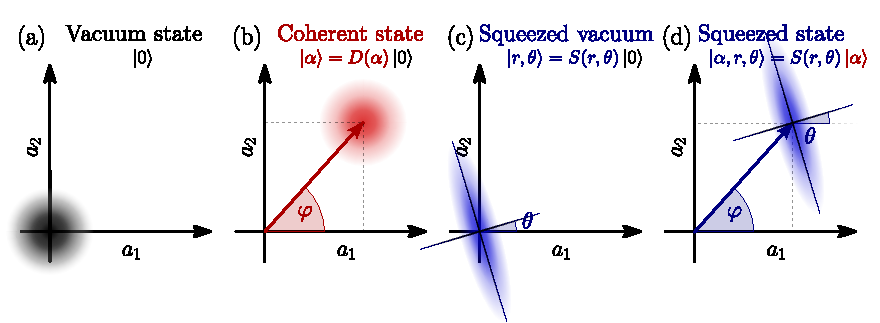
\includegraphics[width=\textwidth]{./chap2/fig/quantumstates (2).pdf}
\caption{Phase-space representations of quantum states and transformations.
(a) Wigner function of the vacuum state: a circular Gaussian centered at the origin, representing equal quantum fluctuations in both quadratures $a_1$ and $a_2$.
(b) Wigner function of a coherent state: a displaced circular Gaussian, showing a shift in phase space along an angle $\varphi$ with unchanged, isotropic noise.
(c) Wigner function of a squeezed vacuum state: an elliptical Gaussian centered at the origin, with reduced noise along a rotated quadrature $X_\theta$ and increased noise in the orthogonal direction.
(d) Wigner function of a displaced squeezed state: an ellipse shifted away from the origin, combining anisotropic fluctuations and a nonzero mean amplitude. The displacement angle $\varphi$ and squeezing angle $\theta$ are independent.} 
\end{figure}

\begin{figure}
\centering
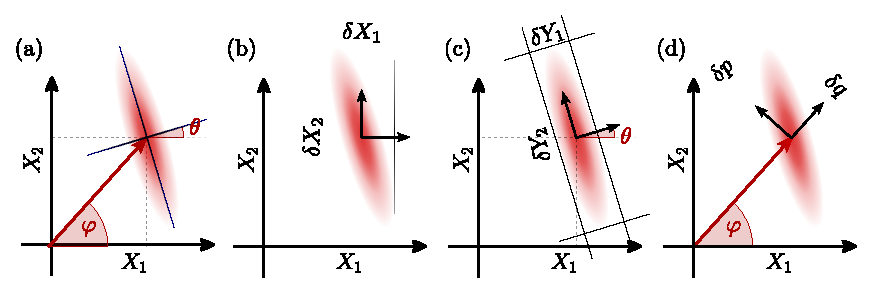
\includegraphics[width=\textwidth]{./chap2/fig/quadratures_phasespace.pdf}
\caption{Phase-space representations of quantum states and transformations.
(a) Wigner function of the vacuum state: a circular Gaussian centered at the origin, representing equal quantum fluctuations in both quadratures $X_1$ and $X_2$.
(b) Wigner function of a coherent state: a displaced circular Gaussian, showing a shift in phase space along an angle $\varphi$ with unchanged, isotropic noise.
(c) Wigner function of a squeezed vacuum state: an elliptical Gaussian centered at the origin, with reduced noise along a rotated quadrature $X_\theta$ and increased noise in the orthogonal direction.
(d) Wigner function of a displaced squeezed state: an ellipse shifted away from the origin, combining anisotropic fluctuations and a nonzero mean amplitude. The displacement angle $\varphi$ and squeezing angle $\theta$ are independent.} 
\end{figure}


We now turn to standard optical quantum states, in particular gaussian states i.e.\ full positive in Wigner functin representations such as coherent and squeezed states, that we will denote in braket notation as $\alpha\rangle$ and  $|\alpha\rangle$ are eigenstates of the annihilation operator:
\begin{equation}
\hat{a}|\alpha\rangle = \alpha|\alpha\rangle
\end{equation}
They can be generated by displacing the vacuum:
\begin{equation}
|\alpha\rangle = \hat{D}|0\rangle, \quad \hat{D}(\alpha) = \exp(\alpha \hat{a}^\dagger - \alpha^* \hat{a})
\end{equation}
They exhibit:
\begin{itemize}
  \item Minimum uncertainty: $\Delta q = \Delta p = 1/\sqrt{2}$
  \item Classical-like dynamics
  \item Poissonian photon statistics
\end{itemize}

\subsection*{Squeezed States}

Squeezed states reduce the variance of one quadrature below vacuum level:
\begin{align}
|\xi_{\omega,\ell}\rangle &= \hat{S}(\xi_{\omega,\ell}) |0\rangle \\
\hat{S}(\xi) &= \exp\left[\frac{1}{2}(\xi^* \hat{a}^2 - \xi \hat{a}^{\dagger 2})\right], \quad \xi = r e^{i\phi}
\end{align}
For phase quadrature squeezing ($\phi = 0$):
\begin{equation}
\Delta q_{\omega,\ell} = e^{-r}/\sqrt{2}, \quad \Delta p_{\omega,\ell} = e^{r}/\sqrt{2}
\end{equation}
Squeezed light is a key resource for precision metrology and quantum information.


\vspace{1em}
This concludes our introduction to the quantum description of light, setting the stage for modelling interactions between quantum optical fields and mechanical resonators.

\subsection{\textcolor{red}{Optical Field Modulations}}
\subsubsection*{Linearization of the Electric Field and Modulation Sidebands}

We consider a single optical mode with a strong coherent drive. The annihilation operator is linearized as:
\begin{equation}
    \hat{a}(t) \to \bar{\alpha}(t) + \delta \hat{a}(t)
\end{equation}
where $\bar{\alpha}(t) \in \mathbb{C}$ is the classical coherent amplitude and $\delta \hat{a}(t)$ captures quantum fluctuations.

The classical part of the electric field is then:
\begin{equation}
    \mathbf{E}_{\text{cl}}(\mathbf{r}, t) = i \sqrt{\frac{\hbar \omega}{2 \varepsilon_0}} \left[
    \mathbf{f}(\mathbf{r})\, \bar{\alpha}(t)\, e^{-i \omega t}
    - \mathbf{f}^*(\mathbf{r})\, \bar{\alpha}^*(t)\, e^{i \omega t}
    \right]
\end{equation}

We now consider two types of sinusoidal modulation at frequency $\Omega$:

\subsubsection*{Amplitude Modulation (AM)}

Let the coherent amplitude be modulated in amplitude:
\begin{equation}
    \bar{\alpha}(t) = \bar{\alpha}_0 \left(1 + \epsilon_a \cos(\Omega t)\right)
    = \bar{\alpha}_0 \left(1 + \frac{\epsilon_a}{2} e^{i\Omega t} + \frac{\epsilon_a}{2} e^{-i\Omega t} \right)
\end{equation}
with $\epsilon_a \ll 1$. The conjugate is:
\begin{equation}
    \bar{\alpha}^*(t) = \bar{\alpha}_0^* \left(1 + \frac{\epsilon_a}{2} e^{i\Omega t} + \frac{\epsilon_a}{2} e^{-i\Omega t} \right)
\end{equation}

Substituting into the field expression:
\begin{align}
    \mathbf{E}_{\text{cl}}^{\text{(AM)}}(\mathbf{r}, t) =
    i \sqrt{\frac{\hbar \omega}{2 \varepsilon_0}} \Big[
    &\mathbf{f}(\mathbf{r})\, \bar{\alpha}_0 \left( e^{-i\omega t} + \frac{\epsilon_a}{2} e^{-i(\omega - \Omega)t} + \frac{\epsilon_a}{2} e^{-i(\omega + \Omega)t} \right) \nonumber \\
    - &\mathbf{f}^*(\mathbf{r})\, \bar{\alpha}_0^* \left( e^{i\omega t} + \frac{\epsilon_a}{2} e^{i(\omega - \Omega)t} + \frac{\epsilon_a}{2} e^{i(\omega + \Omega)t} \right)
    \Big]
\end{align}

\subsubsection*{Phase Modulation (PM)}

Now consider phase modulation of the coherent amplitude:
\begin{equation}
    \bar{\alpha}(t) = \bar{\alpha}_0 e^{i \epsilon_\phi \cos(\Omega t)}
    \approx \bar{\alpha}_0 \left(1 + i \epsilon_\phi \cos(\Omega t)\right)
    = \bar{\alpha}_0 \left(1 + \frac{i \epsilon_\phi}{2} e^{i\Omega t} + \frac{i \epsilon_\phi}{2} e^{-i\Omega t} \right)
\end{equation}
and
\begin{equation}
    \bar{\alpha}^*(t) \approx \bar{\alpha}_0^* \left(1 - \frac{i \epsilon_\phi}{2} e^{i\Omega t} - \frac{i \epsilon_\phi}{2} e^{-i\Omega t} \right)
\end{equation}

Substituting into the field:
\begin{align}
    \mathbf{E}_{\text{cl}}^{\text{(PM)}}(\mathbf{r}, t) =
    i \sqrt{\frac{\hbar \omega}{2 \varepsilon_0}} \Big[
    &\mathbf{f}(\mathbf{r})\, \bar{\alpha}_0 \left( e^{-i\omega t} + \frac{i \epsilon_\phi}{2} e^{-i(\omega - \Omega)t} + \frac{i \epsilon_\phi}{2} e^{-i(\omega + \Omega)t} \right) \nonumber \\
    - &\mathbf{f}^*(\mathbf{r})\, \bar{\alpha}_0^* \left( e^{i\omega t} - \frac{i \epsilon_\phi}{2} e^{i(\omega - \Omega)t} - \frac{i \epsilon_\phi}{2} e^{i(\omega + \Omega)t} \right)
    \Big]
\end{align}

\subsection*{Interpretation}

In both cases, the field contains a carrier at frequency $\omega$ and two sidebands at $\omega \pm \Omega$. Amplitude modulation results in sidebands that are in phase with the carrier, while phase modulation produces sidebands with a $\pm \pi/2$ phase shift relative to the carrier.

\subsection{Quantum Noise and Uncertainty}
\subsection{Sideband Representation}
\hspace{1pt}

\section{Optical Cavities: Basics}
\subsection{Cavity types and Resonance Conditions}
\subsection{Spatial and Longitudinal Modes}
\subsection{Static and Dynamical effects}
\hspace{1pt}

\section{\texorpdfstring{\color{red}Optical Cavities: Three Mirror Cavities}{Optical Cavities: Three Mirror Cavities}}
\subsection{}
\hspace{1pt}

\section{Cavity Optomechanics}
\subsection{Radiation Pressure Coupling}
\subsection{Quantum Langevin Equations}
\subsection{\texorpdfstring{Mechanical Resonators}{Mechanical Resonators}}
\subsection{Noise spectra}
\subsection{\texorpdfstring{\color{red} Three Mirror Cavities as Novel Optomechanical Systems}{Three Mirror Cavities as Novel Optomechanical Systems}}
\hspace{1pt}

\section{Squeezed Light Theory}
\subsection{Single-mode Squeezing}
\subsection{Noise Spectra }
\subsection{Frequency-dependent Squeezing and its use}
\hspace{1pt}

\section{Numerical Methods and Simulations}

lets write smth here 


\chapter{Theory: Frequency Dependent Squeezing \& Membrane based Optomechanics}
This chapter will cover the elementary concepts required to describe an membrane based optomechanical system in a quantum regime. We will first recall basics on optical field quantization as well describing coherent and squeezed light field, to then turn to the more specific frequency dependent squeezed light field. Secondly, we will cover the mathematical description of a mechanical resonator interacting with a generic coherent optical field, highlighting the differences with the seminal optomechanical system of a mirror on a spring. Finally, we will derive the equations of motions of a membrane based optomechanical system with frequency dependent squeezed optical fields. 
\newpage
\minitoc
\newpage


\section{Squeezed Light and Optomechanics}

We will now introduce the concept of Standard Quantum Limit (SQL) in the context of optomechanical measurements, and show how frequency dependent squeezed light can be used to surpass this limit. \\ 

For the rest of this section we will assume the following
\begin{itemize}
  \item A cavity on resonance: $\Delta=0$.
  \item A single port optomechanical cavity: $\kappa_1 \sim \kappa$ .
  \item The unresolved sideband regime: $(\Omega, \Omega_m) \ll \kappa/2$.
\end{itemize}
\subsection{Standard Quantum Limit}
The question of interest is now:
\begin{center}
  \textbf{what is the best displacement sensitivity one can achieve?}
\end{center}  

We start by recalling the reflected phase fluctuation of an optomechanical cavity from section II.2.5 under the aforementioned assumptions:
\begin{equation*}
\delta \hat{q}_r[\Omega] = \, \delta \hat{q}_{\mathrm{in}}[\Omega]  + \mathcal{K}[\Omega]\, \delta \hat{p}_{\mathrm{in}}[\Omega] \quad  \text{with} \quad \mathcal{K}[\Omega] = \frac{\mathcal{C}^2}{2}   \,\hbar  \chi[\Omega] =  \dfrac{128 \mathcal{F}^2 \bar I_{\rm in}}{\lambda^2}  \,  \hbar  \chi[\Omega]
\end{equation*}
where $\mathcal{C}$ is now positive and frequency independent. The resulting reflected phase spectrum reads
\begin{equation*}
  S_{qq}^{r}[\Omega] = S_{qq}^{\rm in}[\Omega] + |\mathcal{K}[\Omega]|^2 S_{pp}^{\rm in}[\Omega] + 2 \, \Re\Big[ \mathcal{K}[\Omega] S_{pq}^{\rm in}[\Omega]\Big]
\end{equation*}

The phase to displacement transduction relation with an optomechanical escape efficiency of 1:
\begin{equation*}
   \delta \hat q_x = \mathcal{C} \delta \hat x [\Omega] = \frac{16 \mathcal{F}\sqrt{\bar I_{\rm in}}}{\lambda}\delta \hat{x}[\Omega]  
\end{equation*}
Using these two relations, we can then express displacement fluctuations in terms of input amplitude and phase fluctuations, assuming the reflected field is a perfect probe of the mechanical resonator position fluctuations i.e. $\delta \hat q_r[\Omega] = \delta \hat q_x[\Omega]$. This treatment is formally equivalent to considering the output phase as a statistical estimator of the position fluctuations being a stationary random process as done in quantum measurement theory \cite{clerk_introduction_2010}. We then write
\begin{equation}
  \delta \hat{x}[\Omega] =\mathcal{C}^{-1} \, \delta \hat{q}_{\mathrm{in}}[\Omega]  + \dfrac{\mathcal{C} }{2} \hbar \chi[\Omega] \, \delta \hat{p}_{\mathrm{in}}[\Omega]
\end{equation}
such that the associated displacement spectrum reads
\begin{equation}
      S_{xx}[\Omega] = \mathcal{C}^{-2} S_{qq}^{\rm in}[\Omega] + \bigg(\dfrac{\mathcal{C} }{2} \hbar |\chi[\Omega]| \bigg)^2 S_{pp}^{\rm in}[\Omega]   + \hbar |\chi[\Omega]| \Re\Big[  e^{i\phi_m[\Omega]} S_{pq}^{\rm in}[\Omega]\Big]
  \label{eq:total_displacement_spectrum}
\end{equation}

We then identify three contributions to the displacement spectrum:
\begin{itemize}
  \item The first term is the laser shot noise (or imprecision noise) scaling inversely with the input power $\bar{I}_\mathrm{in}$, arising from the input phase fluctuations $S_{qq}^{\rm in}[\Omega]$ and given by
  \begin{equation}
    S_{xx}^{\rm SN}[\Omega] = \dfrac{\lambda^2}{256 \mathcal{F}^2 \bar{I}_\mathrm{in}} S_{qq}^{\rm in}[\Omega]
  \end{equation}
  \item The second term is the radiation pressure noise (or backaction noise) scaling linearly with the input power $\bar{I}_\mathrm{in}$, arising from the input amplitude fluctuations $S_{pp}^{\rm in}[\Omega]$ driving the mechanical resonator via radiation pressure given by 
  \begin{equation}
    S_{xx}^{\rm RPN}[\Omega] = \, \dfrac{64 \mathcal{F}^2 \bar{I}_\mathrm{in}}{\lambda^2}\hbar^2 |\chi[\Omega]|^2 S_{pp}^{\rm in}[\Omega]
  \end{equation}
  \item The third term is a correlation term between amplitude and phase fluctuations $S_{pq}^{\rm in}[\Omega]$, which can be non-zero for arbitrary squeezed states as seen in the previous section and given by
  \begin{equation}
    S_{xx}^{\rm cor}[\Omega] = \hbar |\chi[\Omega]|\Re\Big[ e^{i\phi_m[\Omega]} S_{pq}^{\rm in}[\Omega]\Big]
  \end{equation}
\end{itemize}
And we write the total displacement spectrum as the sum of these three contributions
\begin{equation}
  S_{xx}[\Omega] = S_{xx}^{\rm SN}[\Omega] + S_{xx}^{\rm RPN}[\Omega] + S_{xx}^{\rm cor}[\Omega]
\end{equation}

We now consider vacuum/coherent fluctuations such that $S_{qq}^{\rm in}[\Omega]=S_{pp}^{\rm in}[\Omega]=1$ and $S_{pq}^{\rm in}[\Omega]=0$, so that the displacement spectrum simplifies to
\begin{equation}
  S_{xx}[\Omega] = \mathcal{C}^{-2}  + \bigg(\dfrac{\mathcal{C} }{2} \hbar |\chi[\Omega]| \bigg)^2
  \label{eq:total_displacement_spectrum}
\end{equation}
and we look at what noise dominates the displacement spectrum around the mechanical resonance $\Omega \sim \Omega_m$. In this frequency range, there are two frequencies at which the displacement noise contributions are equal, given by the condition $S_{xx}^{\rm SN}[\Omega] = S_{xx}^{\rm RPN}[\Omega]$, leading to the frequency $\Omega_{\text{SQL}}$ defined as
\begin{equation}
  \Omega^{\pm}_{\text{SQL}}  =\;\sqrt{\Omega_m^2-\dfrac{\Gamma_m^2}{2}
\;\pm\;\dfrac{1}{2}\sqrt{\Gamma_m^4-4\Gamma_m^2\Omega_m^2+\Big(\frac{\hbar \mathcal{C}^2}{m }\Big)^2}}
\end{equation}
and consistent with the LIGO/Virgo notation \cite{harry_advanced_2010, aasi_enhanced_2013}. Over the frequency range of interest $\Omega \in [\Omega_m - \Omega_{\text{SQL}}, \Omega_m + \Omega_{\text{SQL}}]$, the displacement noise is dominated by the radiation pressure noise, while outside this range, the noise is dominated by the shot noise. However, for every sideband frequency, there exists an optimal input power $\bar{I}_\mathrm{in}^{\rm SQL}[\Omega]$ at which both contributions are equal, minimizing the total displacement noise. This limit is called the Standard Quantum Limit (SQL) and is a direct consequence of Heisenberg's uncertainty principle applied to continuous position measurements \cite{braginsky_quantum_1992, clerk_introduction_2010}. This SQL intensity is given by
\begin{equation}
  S_{xx}^{\rm SN}[\Omega] = S_{xx}^{\rm RPN}[\Omega] \implies \bar{I}_\mathrm{in}^{\rm SQL}[\Omega] = \dfrac{\lambda^2}{128\mathcal{F}^2 \hbar |\chi[\Omega]|}
\end{equation}
such that plugging back in this SQL intensity in \eqref{eq:total_displacement_spectrum} gives the SQL displacement spectrum as
\begin{equation}
  S_{xx}^{\rm SQL}[\Omega] = \hbar |\chi[\Omega]| \implies S_{xx}^{\rm SN}[\Omega] + S_{xx}^{\rm RPN}[\Omega] \geq \hbar |\chi[\Omega]|
\end{equation}
which is the fundamental limit to continuous position measurements with coherent light. We also note that for high Q resonators, $\Omega_{SQL} \gg \Gamma_m$, so approximating the succeptibility by its real part holds over a relatively large frequency range but fails at resonance where the succeptibility is purely imaginary.

\subsubsection{Thermal Noise}
Thermal noise is a major limitation in optomechanical experiments, as it can mask the quantum effects one aims to observe. The mechanical resonator is indeed coupled to a thermal bath at temperature $T$, which drives the resonator into a thermal state with mean phonon occupation number $\bar n_{\mathrm{th}} = k_B T / (\hbar \Omega_m)$ in the high temperature limit $k_B T \gg \hbar \Omega_m$. The position fluctuations induced by this thermal force is given by
\begin{equation}
  S_{xx}^{\mathrm{th}}[\Omega] = \dfrac{2\hbar}{1 - e^{-\hbar \Omega / k_B T}} \Im \chi[\Omega] \simeq 2 m \Gamma_m k_B T |\chi[\Omega]|^2 \quad \text{if} \quad k_B T \gg \hbar \Omega
\end{equation}
where we used the identity $\Im \chi[\Omega] = m\Gamma_m \Omega |\chi[\Omega]|^2$. At $T=0K$, this reduces to the zero point fluctuations spectrum $S_{xx}^{\mathrm{ZPF}}[\Omega] =\, m \Gamma_m \hbar \Omega_m  |\chi[\Omega]|^2 < $$S_{xx}^{\rm SQL}[\Omega]$, such that is often neglected in the total displacement spectrum. However, at finite temperature, the thermal noise can be much larger than the SQL. Therefore, the total displacement spectrum now reads
\begin{equation}
  S_{xx}[\Omega] = S_{xx}^{\rm SN}[\Omega] + S_{xx}^{\rm RPN}[\Omega] + S_{xx}^{\rm cor}[\Omega] + S_{xx}^{\mathrm{th}}[\Omega]
\end{equation}
In order to experimentally probe these quantum limits without being limited by various technical noises, one would then need: 
\begin{itemize}
  \item A high finesse cavity, such that the shot noise $S_{xx}^{\rm SN} \propto \mathcal{F}^{-2}$ level is low, and the radiation pressure noise $S_{xx}^{\rm RPN} \propto \mathcal{F}^{2}$ is high. One should however ensure the cavity bandwidth $\kappa$ is still much larger than the mechanical frequency $\Omega_m$. This can be ensure tuning the cavity length $L$ and mirror transmissions.
  \item A low mass, low frequency, high quality factor mechanical resonator, such that the susceptibility modulus at resonance $|\chi[\Omega_m]|=Q/m \Omega_{m}^2$ is high, and it comes out of the shot noise level significantly. 
  \item A low temperature environment, such that the thermal noise $S_{xx}^{\mathrm{th}} \propto T$ is low and does not mask the quantum effects. This can be ensured by cryogenic cooling of the mechanical resonator, as well as using high quality factor resonators to reduce the mechanical linewidth $\Gamma_m$.
\end{itemize}

\begin{figure}
  \centering
  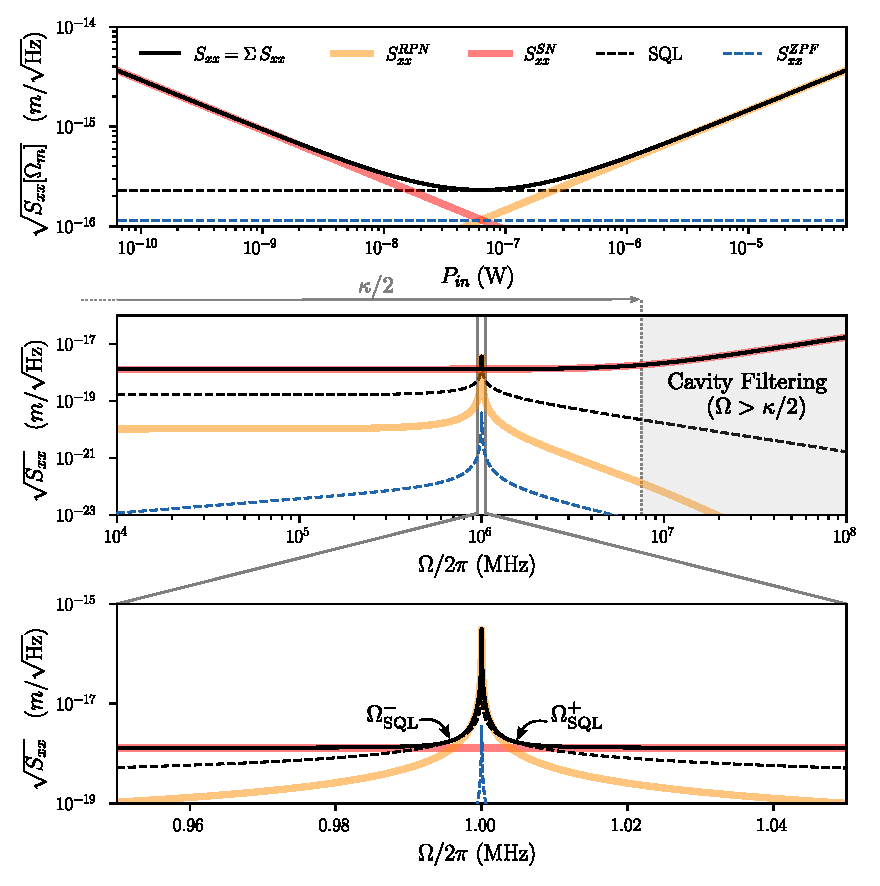
\includegraphics[width=\textwidth]{./chap3/fig/SQL0.pdf}
  \caption{DYes}
  \label{fig:freq_indep_squeezing}
\end{figure}

We now want to derive the displacement spectrum of an optomechanical system driven by a squeezed light field, whether frequency independent or dependent. 

\subsection{Frequency Independent Squeezing in Optomechanical Cavities}
We first recall the (idealized) covariance matrices for both a phase squeezed field and an amplitude squeezed field 
\begin{equation*}
  \mathbf{S}^{0}_{\rm OPO}[\Omega] = 
  \begin{pmatrix}
    e^{+2r} & 0\\
    0 & e^{-2r}
  \end{pmatrix}, \quad
  \mathbf{S}^{\pi}_{\rm OPO}[\Omega] = 
  \begin{pmatrix}
    e^{-2r} & 0\\
    0 & e^{+2r}
  \end{pmatrix}
\end{equation*}
For a phase squeezed field, the displacement spectrum reads
\begin{equation}
  S_{xx}^{0}[\Omega] =   \mathcal{C}^{-2}  e^{-2r} + \bigg(\dfrac{\mathcal{C} }{2} \hbar |\chi[\Omega]| \bigg)^2 e^{+2r}
\end{equation}
while for an amplitude squeezed field, the displacement spectrum reads
\begin{equation}
  S_{xx}^{\pi}[\Omega] =  \mathcal{C}^{-2}  e^{+2r} + \bigg(\dfrac{\mathcal{C} }{2} \hbar |\chi[\Omega]| \bigg)^2 e^{-2r}
\end{equation}
We then see that phase squeezing reduces the shot noise contribution but increases the radiation pressure noise contribution, while amplitude squeezing reduces the radiation pressure noise contribution but increases the shot noise contribution. The input cross correlations being zero, this completely equivalent to the coherent state with a rescaled input intensity $e^{\pm 2r} \bar{I}_\mathrm{in} $ (hidden in $\mathcal{C}$) for phase/amplitude squeezing respectively.
However, neither of these two configurations can reduce both contributions simultaneously, and therefore cannot improve the SQL limit. This is illustrated in figure \ref{fig:freq_indep_squeezing}. 

Now consider an input squeezed state with a frequency independent squeezing angle $\theta=\pi/4$ with covariance matrix
\begin{equation*}
  \mathbf{S}^{\pi/4}_{\rm OPO}[\Omega] = \begin{pmatrix}
         \cosh 2r   & -\sinh 2r  \\[10pt]
        -\sinh 2r  & \cosh 2r  
      \end{pmatrix}.
\end{equation*}
The resulting displacement spectrum then reads
\begin{equation}
  S_{xx}^{\pi/4}[\Omega] = \Bigg(\mathcal{C}^{-2}  + \bigg(\dfrac{\mathcal{C} }{2} \hbar |\chi[\Omega]| \bigg)^2\Bigg)\cosh 2r - \hbar |\chi[\Omega]| \sinh 2r \cos \phi_m[\Omega]
\end{equation}
and we seek the frequency range where the displacement spectrum is below the SQL, i.e. $S_{xx}^{\pi/4}[\Omega] < S_{xx}^{\rm SQL}[\Omega]$. This condition is satisfied when
\begin{equation}
  \tanh r < \cos \phi_m[\Omega] < 1
\end{equation}
Because $\tanh r$ tends to 1 as $r$ increases, the frequency range where the displacement spectrum is below the SQL decreases with increasing squeezing factor $r$. Furthermore, due to the interplay between quadrature correlations and the projection of the $\pi/4$ ellipse onto the output quadrature axis, acting as an effective increase of the shot noise floor with effective intensity $\bar{I}_\mathrm{in} \cosh^{-1} r $, there is an effective range of $r$ above which the displacement spectrum is always above the SQL (for a fixed input intensity). This is illustrated in figure \ref{fig:freq_indep_squeezing}.

Additionally, and as seen in Fig ..., the optimal angle to maximally reduce the displacement spectrum varies with frequency, being 0 at frequencies outside the resonator's bandwidth, $\pi/2$ at the mechanical resonance frequency $\Omega_m$, and about $\pm\pi/4$ at $\Omega_m \pm \Omega_{\rm SQL}$. \\

This motivates the use of frequency dependent squeezed states to reduce the displacement spectrum below the SQL over a broad frequency range, where every sideband frequency needs to be rotated by a different angle to minimize the displacement spectrum. More specifically, sideband noises contributing to both shot noise and radiation pressure noise need to be correlated in a frequency dependent manner to optimally cancel the total displacement noise in the vicinity of the mechanical resonance. 

\subsection{Frequency Dependent Squeezing in Optomechanical Cavities}
We now consider a squeezed state with a frequency dependent angle whose covariance matrix is given by
\begin{equation*}
      \mathbf{S}^{\theta}_{\rm OPO}[\Omega] =\begin{pmatrix}
         \cosh 2r  + \sinh 2r \, \cos 2\theta[\Omega]  & -\sinh 2r \, \sin 2\theta[\Omega]  \\[10pt]
        -\sinh 2r \, \sin 2\theta[\Omega]  & \cosh 2r  - \sinh 2r \, \cos 2\theta[\Omega] 
      \end{pmatrix}
\end{equation*}
The resulting displacement spectrum then reads
\begin{equation}
  \begin{split}
      S_{xx}[\Omega] = & \, \mathcal{C}^{-2} (\cosh 2r  - \sinh 2r \, \cos 2\theta[\Omega])\\
      & +  \bigg(\dfrac{\mathcal{C} }{2} \hbar |\chi[\Omega]| \bigg)^2( \cosh 2r  + \sinh 2r \, \cos 2\theta[\Omega]) \\
      & - \hbar |\chi[\Omega]| \sinh 2r \, \sin 2\theta[\Omega] \, \cos \phi_m[\Omega]
  \end{split}
\end{equation}
As shown in the annex, picking the squeezing angle as
\begin{equation}
  2 \theta[\Omega] = \arctan \Big[\dfrac{2|\mathcal{K}[\Omega]|\cos \phi_m[\Omega]}{1 - |\mathcal{K}[\Omega]|^2}\Big]
\end{equation}
minimizes the displacement spectrum at every sideband frequency, leading to
\begin{equation}
\begin{split}
  S_{xx}[\Omega] = & \cosh 2r \Bigg(\mathcal{C}^{-2}  + \bigg(\dfrac{\mathcal{C} }{2} \hbar |\chi[\Omega]| \bigg)^2\Bigg)  \\
  & -  \sinh 2r \sqrt{\Bigg(\mathcal{C}^{-2}  - \bigg(\dfrac{\mathcal{C} }{2} \hbar |\chi[\Omega]| \bigg)^2\Bigg)^2 + \bigg(\hbar |\chi[\Omega]|\cos \phi_m[\Omega]\bigg)^2}.
\end{split}
\end{equation}
This broadband reduction of the displacement spectrum below the SQL is illustrated in figure \ref{fig:freq_dep_squeezing}. However, for a resonant optomechanical cavity i.e. $\Delta=0$, it is impossible to beat the SQL at the mechanical resonance, where the succeptibility is purely imaginary $\phi_m[\Omega_m] = \pi/2$. \\ 

\begin{figure}
  \centering
  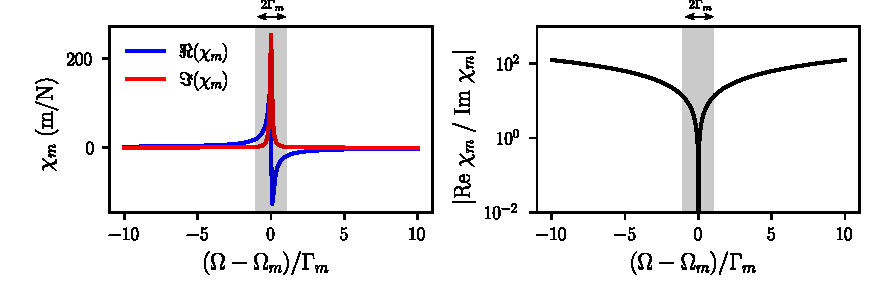
\includegraphics[width=\textwidth]{./chap3/fig/chi_meca.pdf}
  \caption{DYes}
  \label{fig:freq_indep_squeezing}
\end{figure}

\noindent \textbf{Convergence to VIRGO/LIGO notation:} We once again show that this general treatment converges to the one used in the context of gravitational wave detectors. In the free mass regime, $\mathcal{K}[\Omega]$ is real, such that $\phi_m[\Omega]=0$. One can then rewrite the optimal squeezing angle as
\begin{equation}
  2 \theta[\Omega] = \arctan \Big[\dfrac{2\mathcal{K}[\Omega]}{1 - \mathcal{K}^2[\Omega]}\Big] = 2 \arctan \mathcal{K}[\Omega]
\end{equation}
where we used the identity $\arctan 2x/(1-x^2) = 2\arctan x \, \, (\text{mod}\, \pi)$, such that this comes down to the expression used in the context of gravitational wave detectors \cite{harry_advanced_2010, aasi_enhanced_2013}. Furthermore, the mechanical frequency and damping rate will be significantly smaller than the $\hbar \mathcal{C}^2/m$ term such that using the free-mass succeptibility $\chi[\Omega] = -1/m \Omega^2$ boils down the the SQL frequency to the known expression
\begin{equation}
  \Omega_{\text{SQL}} = \sqrt{\dfrac{\hbar \mathcal{C}^2}{2 m }} \implies \mathcal{K}[\Omega] = \Big( \dfrac{\Omega_{\text{SQL}}}{\Omega}\Big)^2
\end{equation}
The displacement spectrum then reduces to the common expression
\begin{equation}
  S_{xx}[\Omega] = \mathcal{C}^{-2} \Bigg( 1  + \Big( \dfrac{\Omega_{\text{SQL}}}{\Omega}\Big)^2 \Bigg)e^{-2r}
\end{equation}
which is the free-mass approximation result used in the GW community. 

\subsection{Filter Cavities for Frequency Dependent Squeezing}

To generate frequency dependent squeezed states, one can use a detuned optical cavity called a filter cavity \cite{kimble_conversion_2001}. The principle is to reflect a frequency independent squeezed state off a single sided detuned cavity, such that only the sidebands resonant with the cavity will undergo a phase shift, effectively rotating the squeezing ellipse by a frequency dependent angle. 
The transfer matrix for a single sideband from a detuned single port cavity was given by
\begin{equation*}
    \kappa \mathrm M_{\Delta}^{-1}[\Omega]  - \mathbf{1} = \begin{pmatrix}
      \dfrac{\kappa/2 + i(\Delta + \Omega)}{\kappa/2 - i(\Delta + \Omega)} & 0 \\[10pt]
      0 & \dfrac{\kappa/2 - i(\Delta - \Omega)}{\kappa/2+ i(\Delta - \Omega)}
    \end{pmatrix}
\end{equation*}


We recall from section II.1.4 that the reflected quadratures from a detuned cavity are given by
\begin{equation*}
    \mathbf{T}_{\mathrm{r}}[\Omega]=  \frac{1}{(\kappa/2 - i\Omega)^{2}+\Delta^{2}}
\begin{pmatrix}
     (\kappa/2)^2 - \Delta^2 + \Omega^2  & - \kappa \Delta  \\[6pt]
    + \kappa \Delta  & ( \kappa/2)^2 - \Delta^2 + \Omega^2 
\end{pmatrix}
\end{equation*}
such that the phase picked up by sidebands at frequency $\Omega$ is given by
\begin{equation}
    \phi_{\mathrm{fc}}[\Omega] = \arctan \Big(\dfrac{2 \Delta \kappa }{\kappa^2/4 - \Delta^2 + \Omega^2}\Big) 
\end{equation}



\section{Cavity Optomechanics with Membrane based systems }
\subsection{Classical Description}
To gain intuition and derive elementary parameters used in the next section, we first describe the classical fields propagating in a three mirror cavity where a membrane with complex amplitude reflection and transmission coefficients \(r_m=|r_m|e^{i\phi_r}\) and \(t_m=|t_m|e^{i\phi_t}\) is placed between two high reflectivity mirrors of amplitude reflection coefficients \( \sim -1 \). The membrane splits the cavity in two sub-cavities of lengths \(L_1\) and \(L_2\), with \(L=L_1+L_2\) the total cavity length. The membrane is initially at mean position $x=0$, and is modelled as a thin dielectric slab of thickness \(d\) and refractive index \(n\), with amplitude reflection and transmission coefficients \(r_m\) and \(t_m\) given by \cite{thompson_strong_2008}
\begin{equation}
r_m = \frac{(n^2-1)\sin k n d}{2 i n \cos k n d  + (n^2+1)\sin k n d}, \qquad t_m = \frac{2 n}{2 i n \cos k n d  + (n^2+1)\sin k n d}. 
\end{equation}
In the lossless case, we will assume the index of refraction $n$ is real, such that \(|r_m|^2 + |t_m|^2 = 1\). The right-moving mean field amplitudes in the left and right sub-cavities are denoted \(\alpha_L\) and \(\alpha_R\), while the left-moving mean field amplitudes are denoted \(\alpha_L'\) and \(\alpha_R'\). The cavity fields are then related by the following equations
\begin{equation}
\begin{split}
\alpha_R  &= t_m \alpha_L + r_m \alpha_R' \\
\alpha_L' &= t_m \alpha_R'+ r_m \alpha_L. \\
\end{split}
\end{equation}

In this case, energy conservation i.e. $|\alpha_L|^2 + |\alpha_R'|^2 = |\alpha_L'|^2 + |\alpha_R|^2$ imposes that $2(\phi_t-\phi_r) = \pi$ such that we can chose $r_m = |r_m|$ and $t_m = i|t_m|$. We rewrite the the cavity fields by injecting the identities $\alpha_L = - \alpha_L' e^{2ikL_1}$ and $\alpha_R' = - \alpha_R e^{2ikL_2}$ leading to
\begin{equation}
   (t_m^2 - r_m^2) e^{ikL} - e^{-ikL}  = 2 r_m \cos(2kL_2 - kL )
\end{equation}
leading to the transcendental equation \cite{jayich_dispersive_2008}
\begin{equation}
  -\cos kL = |r_m|\cos (2kL_2 - kL)
\end{equation}

\subsubsection{Resonance Frequencies}
Following the method in Sankey et al. \cite{sankey_strong_2010}, we now proceed to derive the cavity resonance frequencies as a function of the membrane position \(x\) around its mean position \(x=0\). We will also always consider a long cavity such that \( L \gg \lambda,x \). The cavity sublenghts considering a non zero mean membrane position are then \(L_1 \rightarrow L_1 +  x\) and \(L_2 \rightarrow L_2 -  x\). We will consider the effect of this displacement on the cavity wavenumbers/frequencies as a perturbation $k(x) = k_N + \delta k(x)$ with $k_N = N \pi/L$, that is the membrane displacement does not change the longitudinal mode index \(N\) but modulates it by at most $\pi/L$ (or equivalently by one free spectral range in the frequency domain). We will omit the x dependency in both $k$ and $\delta k$ for ease of notation. It then follows than terms in $k\, L$ and $k\, x$ can be expanded as
\begin{equation*}
    \cos \big( k \, L \big)  = (-1)^N \cos \big( \delta k \,L \big) \quad \text{and} \quad      \cos \big( k \, x \big)  \sim \cos \big( k_N \,  x \big)  
\end{equation*}

such that the transcendental equation becomes
\begin{equation}
  \begin{split}
  (-1)^{N+1} \cos \big( \delta k \,L \big) = |r_m|\cos (k_N \,\delta L) \Big[ &\cos( \delta k \,  \delta L) \cos (2 k_N\, x) \\ 
  & +  \sin(\delta k \,  \delta L) \sin(2 k_N x) \Big]  
  \end{split}
\end{equation}
with $\delta L = L_1 - L_2$ and where we simplified the sines terms already equal to zero. 

We now two consider cases : the historical Membrane In the Middle (MIM) model where $L_1 \sim L_2 \sim L/2 \rightarrow \delta L = 0 $, and the less studied Membrane At The Edge (MATE) model where $L_1 \sim L \gg L_2 \rightarrow \delta L \sim L$. Solving for $\delta k$ in both cases and reinjecting in the dispersion relation $\omega_c(x) = c k(x)$ leads to
\begin{equation}
  \begin{split}
    \text{MIM:} \quad \omega_c(x) & \simeq \omega_{FSR} \Bigg(N  + \frac{1}{\pi} \arccos( (-1)^{N+1}|r_m| \cos 2 k_N  x) \Bigg) \\
    \text{MATE:} \quad \omega_c(x) & \simeq \omega_{FSR} \Bigg( N  + \frac{c}{L} \arctan \bigg( -  \dfrac{1 + |r_m|\cos 2 k_N  x}{|r_m|\sin 2 k_N x} \bigg)\Bigg)
  \end{split}
\end{equation}
When is laser is resonant with the cavity, we then substitute $N \omega_{FSR}$ and $k_N$ by $\omega_0$ and $k$ the laser angular frequency and wavenumber. Taking the derivatives of these resonance frequencies with respect to the membrane position \(x\) then gives the linear dispersive optomechanical coupling \(G = \partial \omega_c/\partial x\) as
\begin{equation}
  \begin{split}
    \text{MIM:} \quad G(x) & =  (-1)^{N+1} \dfrac{2 |r_m|  k_N \omega_{FSR}}{\pi} \dfrac{\sin( 2 k_N  x)}{\sqrt{1 - |r_m|^2 \cos^2( 2 k_N  x)}} \\
    \text{MATE:} \quad G(x) & = \dfrac{2 |r_m|  k_N \omega_{FSR}}{\pi}  \dfrac{|r_m|  + \cos( 2 k_N  x)}{1 + |r_m|^2 - 2 |r_m| \cos( 2 k_N  x)}
  \end{split}
\end{equation}
\subsubsection{Cavity Linewidth and Finesse}

\subsection{Quantum Langevin Equations}

Using the same tools as in section II.2, we can derive the QLE of a membrane based optomechanical system. The transmissive membrane splits the cavity in two sub-cavities of lengths \(L_1\) and \(L_2\), with \(L=L_1+L_2\) the total cavity length. The membrane position operator is described by annihilation operator $\hat x \propto \hat c + \hat c^{\dagger} $ as in the previous section. The central difference with the standard book-keeping optomechanical system of a mirror on a spring is that the membrane splits the cavity in two sub-cavities, such that two bosonic operators \(\hat a_L\) and \(\hat a_R\) are required to describe the intracavity fields. The membrane position then modifies the resonance frequencies of the two subcavities, such that they both depend on the membrane position as \(\omega_L(x)\) and \(\omega_R(x)\) but with inverse trend: when one cavity shortens and its FSR increases, the other lengthens and its FSR decreases. To first order, we can linearize the resonance frequencies as
\begin{equation}
\omega_L(\hat x) \simeq \omega_{L,0} + G_L \hat x, \qquad \omega_R(\hat x) \simeq \omega_{R,0} + G_R \hat x,
\end{equation}
with \(G_L = \omega_{L,0}/L_1\) and \(G_R = - \omega_{R,0}/L_2\) the optomechanical couplings of the two subcavities, and where \(\omega_{L,0}\) and \(\omega_{R,0}\) are the unperturbed resonance frequencies of the two subcavities. 
The system now features a network of optical modes varying linearly with the membrane position, coupled by the membrane transmission. The Hamiltonian of this system can then be written as 
\begin{equation}
  \begin{split}
    \hat{H} = & \,  \hbar \, \omega_{L,0} \, \hat a_L^\dagger \hat{a}^{\vphantom{\dagger}}_L + \hbar \, \omega_{R,0} \, \hat{a}_R^\dagger \hat{a}_R^{\vphantom{\dagger}} + + \hbar \, \Omega_m \hat c^\dagger \hat c \\
    & + \hbar \,  (G_L \,  \hat a_L^\dagger \hat{a}_L^{\vphantom{\dagger}} + G_R \, \hat a_R^\dagger \hat{a}_R^{\vphantom{\dagger}}) \,  \hat x  \\
    & - \hbar \, J(\hat{a}_L^\dagger \hat{a}_R^{\vphantom{\dagger}} + \hat{a}_R^\dagger \hat{a}_L^{\vphantom{\dagger}})  
  \end{split}
\end{equation}
where we only considered one cavity mode per subcavity, and where \(J\) is the photon tunneling rate through the membrane, proportional to the membrane transmission \(t_m\). The first line describes the free evolution of the two subcavity modes and the mechanical resonator, the second line describes the optomechanical interaction between the membrane position and the two subcavity modes, while the third line describes the photon tunneling through the membrane. As before, the commutation relations are given by 
\begin{equation*}
  [\hat a_L^{\vphantom{\dagger}}, \hat a_L^\dagger] = [\hat a_R^{\vphantom{\dagger}}  , \hat a_R^\dagger] = [\hat c, \hat c^\dagger] = 1 \quad \text{and} \quad [\hat a_L^{\vphantom{\dagger}}, \hat a_R^{\vphantom{\dagger}}] = [\hat a_L^{\vphantom{\dagger}},\hat a_R^{\dagger}]  = 0
\end{equation*}
So the commuatators of the Hamiltonian are given by
\begin{equation*}
  [\hat{H}, \hat a_L] = - \hbar (\omega_{L,0} + G_L \hat x) \hat a_L + \hbar J \hat a_R, \quad [\hat{H}, \hat a_R] = - \hbar (\omega_{R,0} + G_R \hat x) \hat a_R + \hbar J \hat a_L
\end{equation*}
and
\begin{equation*}
  [\hat{H}, \hat c] = - \hbar \Omega_m \hat c - \hbar (G_L \hat a_L^\dagger \hat a_L + G_R \hat a_R^\dagger \hat a_R)/x_{\mathrm{ZPF}}
\end{equation*}


\subsubsection{Classical Description : Closed cavity model}
We start by describing the classical behaviour of the cavity. Considering a high finesse cavity, with high reflectivity mirrors \(r_1, r_2 \approx 1\), the cavity fields are written as 
\begin{equation}
\begin{aligned}
\alpha_1 = \alpha_1'
\end{aligned}
\end{equation}
where \(E_{\mathrm{in}}\) is the input field, \(E_1\) the intracavity field before the membrane, \(E_2\) the intracavity field after the membrane, \(E_3\) the transmitted field and \(E_4\) the reflected field. The cavity resonance frequencies are then obtained by solving these equations in the absence of input field \(E_{\mathrm{in}}=0\), leading to the transcendental equation \cite{jayich_dispersive_2008}



We describe the subcavity modes by annihilation operators \( \hat a_1\) and \(\hat a_2\), with unperturbed resonance frequencies \(\omega_1\) and \(\omega_2\). The membrane position operator is described by annihilation operator $\hat x \propto \hat c + \hat c^{\dagger} $ as in the previous section. Considering how the membrane position under the effect of radiation pressure modifies the resonance frequencies of the two subcavities, the subcavity length can be written as \(L_1 = L_{1,0} +  x\) and \(L_2 = L_{2,0} -  x\), with \(L_{1,0}\) and \(L_{2,0}\) the equilibrium lengths, and $x$ the mean static displacement of the membrane. This mean displacement being small compared to the cavity length, we can linearize the resonance frequencies as
\begin{equation}
\omega_1(x) \simeq \omega_{0} + G_1 x, \qquad \omega_2(x) \simeq \omega_{0} - G_2 x,
\end{equation}
with \(G_1 = \omega_{0}/L_{1,0}\) and \(G_2 = \omega_{0}/L_{2,0}\) the optomechanical couplings of the two subcavities, and where \(\omega_{0}\) is the common frequency of the two modes i.e. \(\omega_{1,0} = \omega_{2,0} = \omega_{0}\). The system now features a network of optical modes varying linearly with the membrane position, coupled by the membrane transmission. The Hamiltonian of the system is then given by \cite{xu_cavity_2016}
\begin{equation}
\hat{H} = \hbar \omega_1(x) \hat a_1^\dagger \hat{a}_1 + \hbar \omega_2(x) \hat{a}_2^\dagger \hat{a}_2 + \hbar g(\hat{a}_1^\dagger \hat{a}_2 + \hat{a}_2^\dagger \hat{a}_1) + \frac{\hat{p}^2}{2m} + \frac{1}{2} m \omega_m^2 \hat{x}^2
\end{equation}


Two configurations are then possible: position the membrane at approximately half the total cavity length \(L/2\), such that \(L_{1,0} \simeq L_{2,0}\) and \(G_1 \simeq G_2\); or position the membrane close to one of the mirrors, such that one subcavity is much shorter than the other, e.g. \(L_{1,0} \gg L_{2,0}\) and \(G_1 \ll G_2\). The first configuration is called the \emph{membrane-in-the-middle} (MIM) configuration, while the second one is called the \emph{membrane-at-the-edge} (MATE) configuration. The MIM configuration has been widely studied in the literature \cite{jayich_dispersive_2008, thompson_strong_2008, sankey_strong_2010, xu_cavity_2016}, and has been used to demonstrate various quantum effects such as ponderomotive squeezing \cite{purdy_observation_2013}, quantum non-demolition measurements of phonon number \cite{sankey_strong_2010}, or ground-state cooling of a mechanical resonator \cite{peterson_laser_2016}. However, the MIM configuration suffers from a low optomechanical coupling rate due to the small value of \(G_{1,2}\), which limits its use for quantum experiments. The MATE configuration has been less studied, but offers a much larger optomechanical coupling rate due to the large value of \(G_1\). This makes it a promising candidate for quantum experiments. In this work, we will focus on the MATE configuration.












































\subsubsection*{Set-up and notation}
We consider a three–mode optical model for a membrane-at-the-edge (MATE) cavity with a \emph{highly transmissive} middle membrane. The long cavity mode is denoted by \(a\); the short cavity contributes two nearby modes, \(b_{+}\) and \(b_{-}\), centered \(\pm \lambda/4\) away in displacement. In the mode basis \((a,b_+,b_-)^\top\) we take (with \(\hbar=1\))
\begin{equation}
\label{eq:H}
\mathbf H=
\begin{pmatrix}
\delta_a & J & -J\\[2pt]
J & \delta_+ & 0\\[2pt]
-\,J & 0 & \delta_-
\end{pmatrix},
\qquad
\begin{aligned}
&\delta_a = r_m G_1\,\Delta x,\\
&\delta_\pm = r_m G_2\!\left(\Delta x \mp \frac{\lambda}{4}\right),
\end{aligned}
\end{equation}
with
\begin{equation}
J=\frac{c\,t_m}{2\sqrt{L_1L_2}},\qquad
t_m^2+r_m^2=1,\qquad
G_1=\frac{\omega_0}{L_1},\qquad
G_2=-\frac{\omega_0}{L_2}.
\end{equation}
Here \(\Delta x\) is the membrane displacement from the symmetry point, \(\lambda\) the optical wavelength, \(t_m\) (\(r_m\)) the middle-membrane amplitude transmission (reflection), and \(L_{1,2}\) the long/short sub-cavity lengths. High transmissivity means \(r_m\ll 1\) while \(J=O(t_m)\) can be sizable.

The exact normal modes are eigenoperators \(A_k=\alpha_k a+\beta_k b_+ + \gamma_k b_-\) obtained from \((\mathbf H-\omega_k\mathbb I)\,(\alpha_k,\beta_k,\gamma_k)^\top=0\). From the lower rows one finds the exact amplitude ratios
\begin{equation}
\label{eq:ratios}
\frac{\beta_k}{\alpha_k}=-\frac{J}{\delta_+-\omega_k},
\qquad
\frac{\gamma_k}{\alpha_k}=+\frac{J}{\delta_--\omega_k}.
\end{equation}
The ``physical'' orange branch in the figures is the one continuously connected to the long-cavity mode \(a\).

\section*{Time-domain adiabatic elimination}
Away from the two avoided crossings at \(\Delta x\approx\pm \lambda/4\), the short-cavity detunings \(|\delta_\pm-\omega|\) are large compared to the coupling:
\begin{equation}
\varepsilon_\pm \equiv \frac{J}{|\delta_\pm-\omega|}\ll 1 .
\end{equation}
The Heisenberg equations generated by \eqref{eq:H} read
\begin{equation}
\label{eq:EOM}
\begin{aligned}
i\dot a &= \delta_a a + J b_+ - J b_-,\\
i\dot b_+ &= \delta_+ b_+ + J a,\\
i\dot b_- &= \delta_- b_- - J a.
\end{aligned}
\end{equation}
The fast spectators \(b_\pm\) can be slaved to the slow variable \(a\) by setting \(\dot b_\pm\simeq 0\) to leading order:
\begin{equation}
\label{eq:slaving}
b_+ \simeq -\frac{J}{\delta_+}\,a,\qquad
b_- \simeq \phantom{-}\frac{J}{\delta_-}\,a.
\end{equation}
Substituting \eqref{eq:slaving} into the \(a\) equation in \eqref{eq:EOM} gives an effective single-mode dynamics
\begin{equation}
\label{eq:ae-effective}
i\dot a = \Bigg[\delta_a - J^2\!\left(\frac{1}{\delta_+}+\frac{1}{\delta_-}\right)\Bigg] a .
\end{equation}
Equation \eqref{eq:ae-effective} shows that, in the dispersive region, the spectators do not acquire population to leading order; they merely induce a frequency (phase) shift of the \(a\) mode of order \(J^2/\delta_\pm\).

If optical losses are included as \(\kappa_a,\kappa_\pm\) (phenomenologically via \(\delta_a\to\delta_a-i\kappa_a/2\) etc.), the same elimination yields
\begin{equation}
\label{eq:ae-loss}
i\dot a = \left[\delta_a-\frac{i\kappa_a}{2} - J^2
\left(\frac{1}{\delta_+ - i\kappa_+/2}+\frac{1}{\delta_- - i\kappa_-/2}\right)\right] a,
\end{equation}
and the validity condition strengthens to \(J\ll \sqrt{\Delta_\pm^2+\kappa_\pm^2/4}\) with \(\Delta_\pm=\Re(\delta_\pm-\omega)\).

\paragraph{Connection to eigenvectors.}
Using \eqref{eq:ratios}, for the branch connected to \(a\) one has \(|\beta/\alpha|,|\gamma/\alpha|=O(\varepsilon_\pm)\ll1\). Thus the \(b_\pm\) weights in the physical eigenoperator are \(O(\varepsilon_\pm^2)\), fully consistent with the slaving picture \eqref{eq:slaving}.

\subsubsection*{Closed form for the physical eigenfrequency}
The exact eigenvalue equation for the orange branch obtained from the first row of \((\mathbf H-\omega\mathbb I)v=0\) together with \eqref{eq:ratios} is
\begin{equation}
\label{eq:selfconsistent}
\omega \;=\; \delta_a - J^2\!\left(\frac{1}{\delta_+ - \omega}+\frac{1}{\delta_- - \omega}\right).
\end{equation}
In the dispersive regime \(|\delta_\pm|\gg |\omega|\) one can set \(\omega\to 0\) in the denominators at first order, giving the explicit approximation
\begin{equation}
\label{eq:omega-phys-first}
\boxed{\;
\omega_{\rm phys}(\Delta x)\;\approx\; r_m G_1\,\Delta x
- J^2\!\left[\frac{1}{r_m G_2(\Delta x-\tfrac{\lambda}{4})}
+\frac{1}{r_m G_2(\Delta x+\tfrac{\lambda}{4})}\right].
\;}
\end{equation}
Combining the two fractions yields a compact dispersive form
\begin{equation}
\label{eq:omega-phys-compact}
\boxed{\;
\omega_{\rm phys}(\Delta x)\;\approx\;
r_m G_1\,\Delta x
-\frac{2J^2}{r_m G_2}\,
\frac{\Delta x}{\Delta x^2-(\lambda/4)^2}\;.
\;}
\end{equation}
Close to the symmetry point \(|\Delta x|\ll \lambda/4\), \eqref{eq:omega-phys-compact} becomes nearly linear:
\begin{equation}
\label{eq:omega-linear}
\boxed{\;
\omega_{\rm phys}(\Delta x)\;\approx\;
\underbrace{\left[r_m G_1+\frac{32J^2}{r_m G_2\,\lambda^2}\right]}_{\text{renormalized slope}}
\,\Delta x .
\;}
\end{equation}
In the usual MATE limit \(L_1\gg L_2\) (hence \(|G_1|\ll |G_2|\)), the second term typically dominates the slope; this analytic form explains the gentle ``tilt'' of the orange branch between the two avoided crossings.

\subsubsection*{Schrieffer--Wolff (block-diagonal) derivation}
For completeness, write \(H=H_0+V\) with
\(
H_0=\mathrm{diag}(\delta_a,\delta_+,\delta_-)
\)
and
\(
V=\begin{psmallmatrix}
0 & J & -J\\ J & 0 & 0\\ -J & 0 & 0
\end{psmallmatrix}.
\)
Let \(S\) be anti-Hermitian satisfying \([H_0,S]=-V\).
A suitable choice is
\begin{equation}
S = 
\begin{pmatrix}
0 & \frac{J}{\delta_a-\delta_+} & -\frac{J}{\delta_a-\delta_-}\\[2pt]
-\frac{J}{\delta_a-\delta_+} & 0 & 0\\[2pt]
\frac{J}{\delta_a-\delta_-} & 0 & 0
\end{pmatrix}.
\end{equation}
The transformed Hamiltonian \(\tilde H=e^{S}He^{-S}=H_0+\frac{1}{2}[S,V]+O(J^3/\Delta^2)\) is block-diagonal to second order, with the \(a\) block
\begin{equation}
\label{eq:SW-effective}
H_{\rm eff}^{(a)}=\delta_a
- J^2\left(\frac{1}{\delta_+-\delta_a}+\frac{1}{\delta_--\delta_a}\right),
\end{equation}
which reduces to \eqref{eq:omega-phys-first} when \(|\delta_\pm|\gg |\delta_a|\). Residual \(a\!\leftrightarrow\!b_\pm\) couplings are suppressed to \(O(J^3/\Delta^2)\).

\subsubsection*{Local avoided crossings (breakdown of elimination)}
Near \(\Delta x\simeq +\lambda/4\), only \(b_+\) is near resonant; the relevant subspace is \((a,b_+)\) with
\begin{equation}
H_{\rm loc}^{(+)}=
\begin{pmatrix}
\delta_a & J\\ J & \delta_+
\end{pmatrix},
\qquad
\Rightarrow\qquad
\omega_{\pm}^{(+)}=\frac{\delta_a+\delta_+}{2}\pm
\sqrt{\left(\frac{\delta_a-\delta_+}{2}\right)^2+J^2}.
\end{equation}
The orange branch is the one connecting continuously to \eqref{eq:omega-phys-compact} away from the crossing. The same holds at \(\Delta x\simeq -\lambda/4\) with \(b_-\).
Adiabatic elimination is invalid in windows where \(\varepsilon_\pm\not\ll1\).

\section*{Validity conditions and practical rule}
The small parameter governing all steps is
\(
\varepsilon_\pm = J/|\delta_\pm-\omega|
\).
With losses,
\(
\varepsilon_\pm=J/\sqrt{\Delta_\pm^2+\kappa_\pm^2/4}
\).
A conservative working criterion is
\begin{equation}
\boxed{\;
\max\{\varepsilon_+,\varepsilon_-\}\lesssim 0.2\!-\!0.3
\quad\Rightarrow\quad
\text{errors in }\omega_{\rm phys}\text{ are }O(\varepsilon^2),\
\text{and }|b_\pm|^2/|a|^2=O(\varepsilon^2).
\;}
\end{equation}

\subsubsection*{Optional bright/dark re-basis}
Defining \(b_s=(b_+-b_-)/\sqrt2\) and \(b_d=(b_++b_-)/\sqrt2\), one finds that \(a\) couples only to the \emph{bright} mode \(b_s\) with strength \(\sqrt2\,J\), while \(b_d\) is dark to first order. In this basis the cubic spectrum becomes a quadratic (for \(a,b_s\)) plus a spectator \(b_d\) whose frequency lies near \(r_m G_2\Delta x\) and mixes weakly via \(O(r_m G_2\lambda/2)\). This re-basis is often convenient for fitting and for visualizing how the orange branch acquires its dispersive tilt.

\paragraph{Summary.}
In a high-\(T\) middle-membrane MATE system, the short-cavity modes are far detuned for most \(\Delta x\). They can be adiabatically eliminated, yielding the explicit orange-branch dispersion
\eqref{eq:omega-phys-compact} (or \eqref{eq:omega-linear} near the center), with controlled accuracy quantified by \(\varepsilon_\pm\). Only in narrow windows around \(\Delta x=\pm\lambda/4\) is a \(2\times2\) avoided-crossing description required.

\subsection{Mechanical Resonators}{Mechanical Resonators}
\subsection{Noise spectra}
We will derive the Hamiltonian formalism of a three mirror cavity, and show how it can be used to describe the optomechanical coupling of a membrane in the cavity.
We now have to consider two optical modes coupled to one another through the membrane transmitivities. The Hamiltonian of the system can be written as:
\begin{equation}
\hat{H} = \hbar \omega_1 \hat{a}_1^\dagger \hat{a}_1 + \hbar \omega_2 \hat{a}_2^\dagger \hat{a}_2 + \hbar g(\hat{a}_1^\dagger \hat{a}_2 + \hat{a}_2^\dagger \hat{a}_1) + \frac{\hat{p}^2}{2m} + \frac{1}{2} m \omega_m^2 \hat{x}^2
\end{equation}
where $\hat{a}_1$ and $\hat{a}_2$ are the annihilation operators of the two optical modes, $\omega_1$ and $\omega_2$ their respective frequencies, $g$ the optomechanical coupling strength, $\hat{p}$ and $\hat{x}$ the momentum and position operators of the membrane, $m$ its mass and $\omega_m$ its mechanical frequency. The optomechanical coupling strength $g$ is defined as:
\begin{equation}
g = \frac{\omega_1}{L} \sqrt{\frac{\hbar}{2 m \omega_m}} \left( T_1 + T_2 \right)
\end{equation}
where $T_1$ and $T_2$ are the transmitivities of the two optical modes through the membrane. The Hamiltonian can be diagonalized by introducing the normal modes of the system, which are the eigenstates of the Hamiltonian. The normal modes can be expressed as:
\begin{equation}
\hat{b}_1 = \frac{1}{\sqrt{2}} \left( \hat{a}_1 + \hat{a}_2 \right), \quad \hat{b}_2 = \frac{1}{\sqrt{2}} \left( \hat{a}_1 - \hat{a}_2 \right)
\end{equation}
The normal modes $\hat{b}_1$ and $\hat{b}_2$ are the symmetric and antisymmetric modes of the system, respectively. The Hamiltonian can then be rewritten in terms of the normal modes as:
\begin{equation}
\hat{H} = \hbar \omega_1 \hat{b}_1
^\dagger \hat{b}_1 + \hbar \omega_2 \hat{b}_2^\dagger \hat{b}_2 + \hbar g(\hat{b}_1^\dagger \hat{b}_2 + \hat{b}_2^\dagger \hat{b}_1) + \frac{\hat{p}^2}{2m} + \frac{1}{2} m \omega_m^2 \hat{x}^2
\end{equation}


\paragraph{Diagonalisation of two non-degenerate, tunnel-coupled optical cavities.}
Let \(a_{1}\) and \(a_{2}\) (with the usual bosonic commutation relations) annihilate photons in the first and second cavity, whose bare resonance frequencies are \(\omega_{1}\neq\omega_{2}\).  Photon tunnelling at rate \(J>0\) through the semi-transparent middle mirror couples the two modes, giving the second-quantised Hamiltonian
\[
H
  =\hbar
    \begin{pmatrix}
      a_{1}^{\dagger} & a_{2}^{\dagger}
    \end{pmatrix}
    \underbrace{\begin{pmatrix}
      \omega_{1} & J\\
      J          & \omega_{2}
    \end{pmatrix}}_{\,\mathbf M}
    \begin{pmatrix}
      a_{1}\\ a_{2}
    \end{pmatrix}.
\]
Diagonalising the \(2\times2\) Hermitian matrix \(\mathbf M\) one finds the normal–mode (super-mode) eigenfrequencies
\begin{equation}
\label{eq:split}
\omega_{\pm}= \frac{\omega_{1}+\omega_{2}}{2}\;\pm\;
              \sqrt{J^{2}+\bigl(\tfrac{\omega_{1}-\omega_{2}}{2}\bigr)^{2}},
\end{equation}
and introduces a mixing angle \(\theta\) via
\[
\tan 2\theta \;=\;\frac{2J}{\,\omega_{2}-\omega_{1}\,}, 
\qquad 0<\theta<\pi/2.
\]
The corresponding canonical operators
\[
A_{+}= \cos\theta\,a_{1}+\sin\theta\,a_{2},
\qquad
A_{-}=-\sin\theta\,a_{1}+\cos\theta\,a_{2},
\]
obey \([A_{\mu},A_{\nu}^{\dagger}]=\delta_{\mu\nu}\) and bring the Hamiltonian to the diagonal form
\[
H=\hbar\omega_{+}\,A_{+}^{\dagger}A_{+}\;+\;\hbar\omega_{-}\,A_{-}^{\dagger}A_{-},
\]
revealing two independent harmonic oscillators whose frequency splitting \(\omega_{+}-\omega_{-}=2\sqrt{J^{2}+[(\omega_{1}-\omega_{2})/2]^{2}}\) interpolates smoothly between the strong-coupling limit (\(\omega_{1}\approx\omega_{2}\)) and the large-detuning regime where each cavity mode retains its individuality and the admixture of its neighbour is suppressed by the small parameter \(J/|\omega_{2}-\omega_{1}|\ll1\).




\chapter{Experimental Methods}
This chapter will cover the experimental methods used in the development of optomechanical systems, focusing on the generation of squeezed light and the techniques for optical locking and quadrature measurement. The methods are designed to enhance the sensitivity of measurements in quantum optics and optomechanics.
\minitoc
\newpage
\section{Optical Locking Techniques with PyRPL}
A central aspect of the experimental setups is the ability to stabilize various optical features. In this work, it is the case for the relative phase between two optical paths, keeping optical cavities on resonance, or fixing the detuning between a master and a slave laser. \newline

\noindent This section will cover the locking techniques used in this work, from basic Michelson-type locking to more advanced Pound-Drever-Hall techniques and phase-locked loops. The implementation of these techniques using the in-house library PyRPL is presented. 

\subsection{Proportion-Integral (PI) Controllers}
Proportional-Integral (PI) controllers are widely used in quantum optics experiments to stabilize critical parameters such as cavity length, laser frequency, and optical phase. To this end, one needs to extract an error signal \( \epsilon(t) \) that quantifies the deviation from a desired setpoint, such as a target temperature, phase difference or cavity resonance. It is typically expressed as the difference between a measured signal and its reference value:
\[
\epsilon(t) = s_{\text{meas}}(t) - s_{\text{ref}},
\]
where \( s_{\text{meas}}(t) \) denotes the physical quantity monitored in the experiment (e.g., reflected intensity or interferometric signal), and \( s_{\text{ref}} \) is the target value corresponding to the lock point.\newline

\noindent For effective feedback stabilization, the error signal must satisfy several essential criteria:
\begin{itemize}
    \item \textbf{High SNR:} Near the setpoint, \( \epsilon(t) \) should exhibit a high SNR to ensure robust locking and minimize the influence of technical and electronic noise.
    \item \textbf{Linearity and antisymmetry:} The error signal should be linear and antisymmetric in a neighborhood of the operating point. Small deviations from the setpoint should produce a proportional response in \( \epsilon(t) \), with opposite signs for deviations of opposite direction.
    \item \textbf{Monotonicity and uniqueness:} The slope \( \partial \epsilon / \partial x \), where \( x \) denotes the control parameter (e.g., cavity length or laser frequency), should be monotonic and unambiguous near the lock point to avoid multiple equilibrium points and ensure stable locking behavior.
    \item \textbf{Steep slope near the setpoint:} A steeper slope improves sensitivity to small deviations and enhances lock accuracy, although it must be balanced against potential noise amplification.
    \item \textbf{Bandwidth compatibility:} The spectral content of \( \epsilon(t) \) must be compatible with the bandwidth of the actuator and the dynamics of the system. For example, in the case of a piezoelectric transducer, which acts as a low-pass mechanical element, the error signal high-frequency components won't be compensated by the actuator.  
\end{itemize}

\noindent The PI controller computes the feedback signal \( u(t) \) from the error signal \( \epsilon(t) \) according to:
\begin{equation}
    u(t) = K_P \, \epsilon(t) + K_I \int_0^t \epsilon(\tau) d\tau
    \tag{III.1}
\end{equation}
where \( K_P \) and \( K_I \) are the proportional and integral gains, respectively. The proportional term \( K_P \, e(t) \) responds to the current error and primarily acts on mid-frequency deviations, enabling rapid corrections. The integral term \( K_I \int \epsilon(\tau) d\tau \) accumulates past errors and is most effective at low frequencies, helping to eliminate long-term drifts and steady-state offsets. \newline

\noindent In classical control theory, PID (Proportional-Integral-Derivative) controllers are designed to stabilize dynamic systems by combining three terms: a proportional term for immediate response, an integral term to eliminate steady-state error, and a derivative term that anticipates future error based on the rate of change. However, in practical experimental setups—particularly in quantum optics—PI control (Proportional-Integral) is typically sufficient and even preferable to full PID control. The derivative term, which acts predominantly at high frequencies, is generally unnecessary and can be counterproductive. This is because the feedback actuator is often a piezoelectric transducer, which exhibits non-zero capacitance. Combined with the finite output impedance of the control electronics, this forms a natural low-pass filter that significantly attenuates high-frequency components of the feedback signal. As a result, any derivative term—which primarily targets high-frequency correction—would be both ineffective due to this filtering and potentially harmful by injecting high-frequency noise into the loop. \newline 

\noindent Therefore, PI control offers a balanced and robust approach: the integral term suppresses low-frequency drifts (typically below a few Hz to tens of Hz), the proportional term corrects intermediate-frequency deviations (up to a few kHz), and high-frequency components (above the mechanical resonance or actuation bandwidth) are naturally filtered out and deliberately left uncorrected. This allows for stable feedback while preserving high-frequency signals—such as thermal noise or mechanical sidebands—which carry essential physical information for analysis and measurement.

\subsection{Temperature Locks}
A first example of a PI lock used in this work is the temperature lock, which is used to stabilize the temperature of non linear crystals embedded inside optical cavities. The error signal is derived from a temperature sensor, such as a thermistor, which measures the temperature of the crystal. The error signal is then fed into a PI controller, which adjusts the heating element, a peltier module in our case, to maintain the desired temperature setpoint. \newline

\noindent The temperature lock is crucial for maintaining the phase matching conditions in nonlinear optical processes (developped in the next section), such as second-harmonic generation or optical parametric oscillation, where the efficiency of frequency conversion depends sensitively on the crystal temperature. By stabilizing the temperature, we ensure that the nonlinear interactions remain optimal, leading to consistent and reproducible results in experiments involving squeezed light generation or other nonlinear optical phenomena. \newline



\subsection{Optical paths Locks}
Controlling the relative path length between two arms of an interferometer is a fundamental technique in quantum optics. The basic idea is to use the interference of light from two paths to lock the phase difference between them. Although not being the same experiental setups, Michelson interferometers, Mach-Zhender interferometers, and Local Oscillator stabilization error signals fall in the same category as they are derived from the same principle. Namely, the error signal is proportional to the sine of the phase difference between the two arms: 
\begin{align}
\epsilon(\Delta \phi) \propto  \sin(\Delta \phi) 
\end{align}
where $\Delta \phi = \phi_a - \phi_b$ is the phase difference between the two optical paths. Analogically, we would need to add an adjustable voltage offset, as to be able to tune the error signal to zero at the desired phase difference, before seeding this error signal to the PI block. Digitally, this is performed by adding a constant offset to the error signal, which can be adjusted to set the desired phase difference. \newline

\noindent In practice, this is implemented by mounting a mirror on which one of the arms is reflected, and then using a piezoelectric transducer to control the position of the mirror, hence modulating the relative phase between the two optical paths. The piezo is then feedback controlled through a PI loop, which adjusts the voltage applied to the piezo to set the error signal to 0. 
FIGURE 

\subsection{Side of Fringe Locks}

\subsection{Pound-Drever-Hall Locks}
Another key technique extensively used in this work is the \textit{Pound-Drever-Hall} (PDH) method, a high-sensitivity scheme for stabilizing either the cavity length to a fluctuating laser frequency, or vice versa. The method relies on imposing phase modulation sidebands on the laser field, typically using an electro-optic modulator (EOM), and using these sidebands as phase-stable references. Because they lie far outside the cavity linewidth (\( \Omega_{\text{mod}} \gg \kappa \)), the sidebands are reflected nearly unchanged: \( r(\omega_\ell \pm \Omega_{\text{mod}}) \approx 1 \). In contrast, the carrier field near resonance acquires a frequency-dependent phase shift upon reflection, captured by the complex cavity reflection coefficient \( r_c(\delta) \). The PDH error signal is obtained by detecting the reflected beam and demodulating the photocurrent at the modulation frequency, isolating the beat terms between carrier and sidebands. The resulting signal is proportional to the \textit{imaginary part} of \( r_c(\delta) \), which varies antisymmetrically with detuning and provides a zero-crossing error signal ideal for linear feedback. This imaginary component encodes the rapid phase dispersion near resonance that allows the system to discriminate the sign and magnitude of frequency deviations. In contrast, the real part of \( r_c(\delta) \), being symmetric around resonance, does not yield a usable error signal. \newline

\noindent The \textit{demodulation phase} plays a critical role in selecting the appropriate quadrature of the signal for feedback. Since the beat signal between the carrier and sidebands has both in-phase (cosine) and quadrature (sine) components, choosing the correct demodulation phase ensures that the extracted error signal aligns with the imaginary part of the reflection coefficient. A misaligned demodulation phase can lead to mixing of the symmetric (real) part into the error signal, thereby reducing sensitivity and introducing offset or distortion near the lock point. In practice, the demodulation phase is optimized empirically---either via a variable phase shifter in the electronic demodulation path or by adjusting the physical delay in the reference oscillator---to maximize the slope of the error signal at zero-crossing, corresponding to pure detection of the dispersive component.
\begin{figure}[htbp]
    \centering
    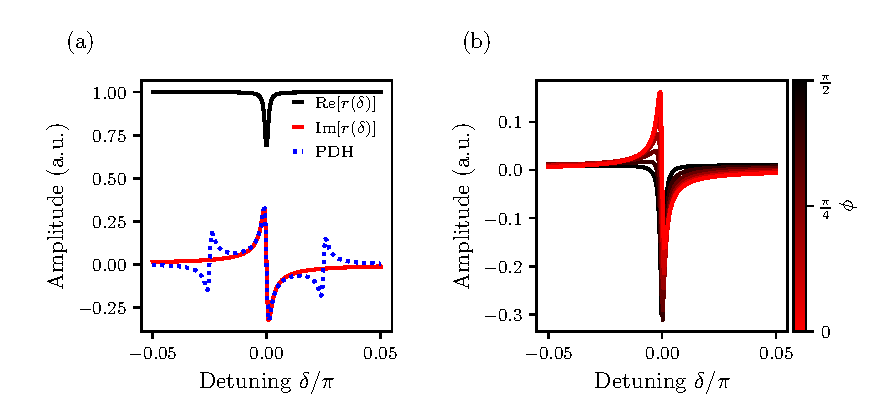
\includegraphics[width=\textwidth]{./chap3/fig/PDHplots.pdf}
    \caption{
        Schematic of the Pound-Drever-Hall (PDH) locking technique. 
        The laser passes through an electro-optic modulator (EOM) generating phase modulation sidebands. 
        The modulated beam is incident on the optical cavity, and the reflected light is detected by a photodiode (PD). 
        The photocurrent is demodulated at the modulation frequency to produce the PDH error signal, which is fed to a PI controller driving the cavity actuator (e.g., piezo). 
        Key components are labeled: EOM (electro-optic modulator), PD (photodiode), LO (local oscillator for demodulation), and PI (proportional-integral controller).
    }\label{fig:PDH_scheme}
\end{figure}

\noindent
The \textit{lock-in optical phase-sensitive error measurement} (LOPSEM) technique is a versatile method for extracting phase information from modulated optical signals. In the context of PDH locking, LOPSEM is used to demodulate the photodiode signal at the modulation frequency, isolating the dispersive error signal required for feedback. By employing a lock-in amplifier or digital demodulation, the technique enables precise selection of the signal quadrature, allowing for robust discrimination of phase shifts induced by cavity detuning. This approach enhances the sensitivity and stability of optical locks, making it an essential tool in quantum optics experiments where accurate phase control is critical.



\subsection{Offset frequency Locks}

coucou Marie 

\subsection{Coherent Sideband Locks}
\subsection{PyRPL Control Implementation}

\section{Optical Cavities and Squeezed Light Generation}
Maybe I need to add a section on the theory of squeezed light generation, but for now I will just focus on the experimental methods.
\subsection{Cavity Types and Alignement Procedures}


\subsection{Bowtie-type Optical Parametric Oscillator (OPO)}
\subsection{Phase Matching and Nonlinear Crystals}
\subsection{Filter Cavities for Squeezing Rotation}

\section{Quadrature Measurement Techniques}
\subsection{Direct Detection with Photodiodes}
\subsection{Balanced Homodyne Detection}
\subsection{Local Oscillator Design and Control}
\newpage


\chapter{Experiments: Optomechanics}
% References are needed for historical context, technical claims, and specific data.
% Suggested [?] placements below:

This chapter will cover the experimental methods used in the development of optomechanical three-mirror cavity systems, focusing on the design, fabrication, and characterization of mechanical resonators within optical cavities. The methods are designed to enhance the sensitivity of measurements in quantum optics and optomechanics.
\minitoc
\newpage 

Over the past two decades, optomechanical systems have greatly benefited from advancements in optical coating technologies, enabling the realization of high-finesse cavities ($\mathcal{F}>10^5$)\cite{coating_review}. Simultaneously, progresses in micro/nanofabrication allowed the making of mechanical structures with high $Q$ factors ($>10^6$)\cite{nanofab_review}. Despite these achievements, a significant challenge remained: fabricating mechanical elements that possess both high $Q$ and high reflectivity, as optical, mechanical and thermal effects often degrade system performance and hinder ultra-sensitive measurements\cite{optomech_challenges}.
\section{System Description and Setup}

\subsection{Previous LKB work and Motivation}

Previous optomechanics experiments at LKB have primarily utilized Fabry--Pérot cavities with two mirrors, where the end mirror of the cavity was typically a HR mirror deposited on top of a mechanical structure featuring a mechanical mode of interest~\cite{}. 
\begin{itemize}
\item Over Aurélien's and Leonard's PhD works, the group in collaboration with ONERA developed a platform based on a $1$-mm-thick quartz micropillar with an effective mass of $33~\mu$g. The structure supports a fundamental compression mode oscillating at $3.6$~MHz, with a mode shape as shown in Fig.~\ref{fig:micropillar_mode}. Using a dry-film photoresist technique, a $100~\mu$m diameter high-reflectivity mirror was deposited on one end of the pillar. Careful design of the suspension has yielded mechanical quality factors up to $3\times 10^{6}$ at room temperature and up to $7\times 10^{7}$ below 1~K. When integrated into a $50~\mu$m-long Fabry--Pérot cavity with a custom-fabricated coupling mirror, finesses exceeding $10^{5}$ were achieved. Importantly, this compact cavity remains robust against vibrations of the dilution refrigerator and maintains alignment during cooldown, thereby providing a stable platform to study optomechanical effects in the intermediate mass regime. \color{red} limitations and why it didnt work \color{black}


\item Then over Rémi's and Michael's PhD, another resonator was developed in collaboration with Francesco Marin’s team, based on a suspended silicon disk. The device operates in a balanced mode, where the central disk vibrates in opposition to four surrounding counterweights. By adjusting the geometry, the resonance frequency was increased to $280$~kHz, corresponding to an effective mass of about $110~\mu$g, bringing the system closer to the micropillar parameters. A HR mirror was then deposited on top using the same technique as the micropillar. Finesse of about $\sim 50 000$ were then reached. At cryogenic temperature, optimized designs reached mechanical quality factors on the order of $1.2 \times 10^{6}$.\color{red} limitations and why it didnt work \color{black}

\end{itemize}

Although the systems ended up being limited by various factors mentioned above (optical, mechanical and thermal effects)~\cite{}, the parts designed over the years did feature a high level of passive stability as well as good thermalization properties.  A pivotal solution, introduced by Regal, Kimble, Harris, and collaborators\cite{Regal2008,Harris2008}, was to decouple these requirements by embedding a high-$Q$ mechanical resonator within a high-finesse optical cavity, using the optical field to probe and control the resonator’s dynamics.

\subsection{Specifications and Design}
It was then decided to build on this design and extend it to a three-mirror cavity in a MATE configuration to benefit from this large linear coupling range as detailed in the previous chapter. That is the work Michael and myself undertook during my M2 internship and the first year of my PhD.
This new three mirror cavity then needed to fulfill various requirements: 
\begin{itemize}
    \item \textbf{High Finesse}: input and back mirrors should both have high reflectivities, with low extra losses such as scattering, absorption, etc ...\cite{AmatoPhD}
    \item \textbf{High $Q$ factor}: the middle mirror i.e. the mechanical resonator, should feature a high $Q$ factor, ideally above $10^6$, in order to ensure a good sensitivity to radiation pressure forces\cite{SiN_review}
    \item \textbf{Optical alignement}: the cavity should be designed to allow for easy optical alignment, with the ability to mode match the setup fairly easily.
    \item \textbf{Dynamical range}: both input and output mirrors should be mounted on piezoelectric actuators, allowing for a dynamic range of at least few microns to scan few FSRs. The piezo actuators should also be able to provide a good bandwidth, ideally above 100 kHz, as well as a sub-nanometer resolution to ensure a good control of the cavity length\cite{piezo_review}.
    \item \textbf{Compactness \& Stability }: the entire assembly should be compact, with a high level of passive stability, yet without mechanically low pass filtering the piezo actuators motion during the locking. 
    \item \textbf{Vacuum and Cryogenic compatibility}: the cavity should be vacuum compatible, and the mirrors should be thermally anchored to the vacuum chamber in order to ensure a good thermalization of the system. Same holds for the cryogenic compatibility, although no test could be performed during this thesis. The cavity was nonetheless designed to be compatible with cryogenic operation.
\end{itemize}
\subsubsection{High Finesse}

Low loss mirrors were produced by \textbf{Jérôme~DEGALLAIX} and \textbf{David~HOFMAN} at the
\textit{Laboratoire des Matériaux Avancés} (LMA, Lyon) using
ion-beam-sputtered (IBS) Bragg stacks made of $\mathrm{Ta_2O_5}$ (high index,
$n\!\approx\!2.09$) and $\mathrm{SiO_2}$ (low index, $n\!\approx\!1.46$)\cite{AmatoPhD,LMA_IBS}. \\
The coatings were deposited in the LMA's \textit{Veeco SPECTOR} chambers and subsequently annealed at 500°C for 10 hours to minimise both optical (absorption) and mechanical losses, following the recipe of Amato \textit{et~al.}\,\cite{AmatoPhD}.
\footnote{Identical optics are used for the Advanced LIGO, Advanced Virgo
and KAGRA interferometers\cite{LIGO_optics}.}.\\

We supplied the LMA with a batch of substrates with various radii of curvature to explore different cavity geometries:
\begin{itemize}
  \item \textbf{Plane substrates:} Laseroptik S--00798
  \item \textbf{Plano-concave substrates:}
    \begin{itemize}
        \item Laseroptik S--00128 ($R = 20$ mm)
        \item Laseroptik S--00127 ($R = 15$ mm)
        \item Laseroptik S--00126 ($R = 10$ mm)
    \end{itemize}
\end{itemize}

All optics feature
\begin{itemize}
  \item \textbf{Back‐side AR:} $R \lesssim 100\,$ppm. This is not critical for the cavity performance since the back side is not actually contributing to the finesse, but it is important to avoid parasitic reflections in the setup.
  \item \textbf{Front‐side HR:}
    \begin{itemize}
        \item[] $T \sim 20 \pm 4\,$ppm on the plane mirrors,
        \item[] $T \sim 50 \pm 10\,$ppm and $100 \pm 10\,$ppm on the
                concave mirrors, respectively,
    \end{itemize}
  \item total round‐trip scatter\,+\,absorption
        $\lesssim 20\,$ppm, in agreement with the measurements reported (absoption $\sim$0.7ppm, scattering $\sim$10ppm)
        in Ref.\,\cite{AmatoPhD}.
\end{itemize}

The quarter‐wave design is centred at $\lambda = 1064$ nm for normal incidence.  After annealing, the measured mechanical loss angle of the $\mathrm{TiO_2\!:\!Ta_2O_5}/\mathrm{SiO_2}$ stack is $\phi < 4\times10^{-4}$ at 1 kHz  \color{red} link to mechanical damping needed \color{black}, supporting cavity finesses in the range $200\,000-500\,000$ before excess scatter or absorption dominates\cite{AmatoPhD}.

\subsubsection{High $Q$ factor}

The middle mirror is a commercially\,–\,available stoichiometric silicon-nitride
(Si$_3$N$_4$) membrane supplied by Norcada (NX10050AS)\cite{SiN_review,Norcada_datasheet}.
It consists of a $1\,\mathrm{mm}\times1\,\mathrm{mm}$, $50\,\mathrm{nm}$-thick
Si$_3$N$_4$ film suspended in a $10\,\mathrm{mm}\times10\,\mathrm{mm}$,
$200\,\mu\mathrm{m}$-thick silicon frame and is marketed specifically for
\emph{high-$Q$} resonator applications. Because stoichiometric LPCVD Si$_3$N$_4$ is under high intrinsic tensile
stress ($\sigma\!\approx\!0.9\;\mathrm{GPa}$), the square drum supports
MHz-frequency modes with exceptionally low mechanical loss\cite{SiN_review}.

\begin{itemize}
  \item \textbf{Room temperature.}  Measurements on nominally identical
        Norcada membranes report quality factors
        $Q \sim 5\times10^{6}$ at $\approx1\,\mathrm{MHz}$ in
        $<10^{-6}$ mbar vacuum \cite{SiN_review,Norcada_datasheet}.
  \item \textbf{Cryogenic operation.}  Cooling to $T \lesssim 300\,\mathrm{mK}$
        reduces internal friction by an order of magnitude, with
        $Q>10^{7}$ routinely observed \cite{SiN_cryogenic}.
\end{itemize}

On the basis of these results we set the following design targets:
\[
  Q_{\mathrm{RT}} \ge 5\times10^{6}, \qquad
  Q_{\mathrm{cryogenic}} \ge 1\times10^{7}.
\]
The membrane’s high stress, thin-film nature and dielectric composition make
it fully compatible with ultra-high-vacuum environments and repeated
cryogenic cycling, while introducing (a priori) negligible optical loss in the cavity.
These attributes ensure a robust, spectrally clean mechanical resonator for
advanced quantum-optomechanics experiments.

\subsubsection{Optical alignment}
The cavity is designed to be compatible with the Thorlabs cage system. The input mirror is mounted on a 3 axis cage mount, allowing for easy alignment of the input mirror with respect to the cavity optical axis. Both the resonator and the back mirror are embedded within a custom-made holder, which is itself integrated into the cage system. The relative tilt between the resonator and the back mirror is adjusted using a set of 3 screws with a very fine thread, allowing for a fine alignment of the parallelism of the back cavity. The alignment procedure is detailed in section~\ref{sec:alignment_procedure}.

\subsubsection{Dynamical range}

The input (front) mirror is glued to a PI \texttt{P-016.00H} ring-stack piezoelectric actuator using vacuum epoxy (Torr Seal). Driven from 0 to $+1000\,\mathrm{V}$ it provides a longitudinal stroke of $5\,\mu\text{m}$, a blocking force of $2.9\,\mathrm{kN}$, as well as an unloaded resonance of 144 kHz, making it suitable for fast, low-noise cavity-length control.

The end-mirror–membrane assembly is mounted on a flexure holder actuated by three \texttt{PD080.31} piezo chips arranged mechanically in series. Each chip yields $2\,\mu\text{m}$ of travel over a drive range of $-20$ to $+100\,\mathrm{V}$; the triple stack therefore supplies roughly $6\,\mu\text{m}$ of coarse tuning while preserving high stiffness and sub-microsecond response.

Combining the $5\,\mu\text{m}$ stroke of the front \texttt{P-016.00H} with the $6\,\mu\text{m}$ range of the rear triple stack provides an overall cavity-length adjustment of about $11\,\mu\text{m}$ — equivalent to more than 20 free spectral ranges — with sub-nanometre resolution when driven by low-noise high-voltage amplifiers.


\subsubsection{Compactness \& Stability}
The entire assembly is built as a cage system using standard Thorlabs cage parts, allowing for a compact and stable assembly\cite{Thorlabs_cage}. The cage system also allows for (relatively) easy alignment of the mirrors, as well as easy access to the piezo actuators.

\subsubsection{Vacuum and Cryogenic compatibility}
The back cavity composed of the back mirror and the middle mirror is embedded inside an Oxygen Free Copper (OFHC) assembly with a circular geometry, eventually mitigating for transverse misalignment issues when going to cryogenic temperatures, the constraints compensating themselves radially with respect to the symmetry axis of the cavity assembly\cite{OFHC_review}. Furthermore, the screws used to hold the assembly together are made of brass with a thermal expansion coefficient lower than that of the OFC, tightening up the cavity when reaching cryogenic temperatures.
Thorlabs cage parts are compatible with moderate vacuum operation down to $\sim 10^{-5} mbar$ if properly degreased and ultrasound cleant, but a custom cryocompatible system to hold the input mirror would be needed for operation at cryogenic temperatures. \\


\begin{figure}[H]
    \centering  
    \includegraphics[width=\textwidth]{./chap5/fig/schéma_cavity.pdf}
    \caption{Cavity design and assembly. (a) The figure shows the overall assembly of the MATE system from various views, highlighting the integration of the high-finesse mirrors, the membrane resonator embedded inside the back cavity copper assembly held to the input mirror Thorlabs holder through a cage system.(b) The exploded view details the arrangement of the mechanical and optical components, illustrating the modular design that facilitates alignment, stability, and compatibility with vacuum environments.}
    \label{fig:cad_cavity}
\end{figure}


The initial design of the cavity was made using Autodesk Fusion 360, allowing for a detailed 3D model of the entire assembly, including the piezo actuators, the mirrors and the cage system. The design was then exported to a STEP file format, which was used to manufacture the parts using a 3 axis CNC milling machine and a digital lathe. The pieces were machined by \textbf{Carounagarane~DORE} and \textbf{Gael~COUPIN} at the LKB mechanical workshop with 100$\mu$m tolerance. A detailed view of the cavity design and assembly is shown in Fig.~\ref{fig:cad_cavity}.

\subsection{Flexure Actuation}

One specificity of the MATE system is that the back cavity is significantly shorter than the front cavity, which would require high precision in both the machining of the copper pieces and the positioning of the resonator. In our case, we aim at a centimetric cavity which would require to position the membrane at roughly hundreds of microns from the back mirror, and parallel to the back mirror. Moving the membrane independently from the back mirror while maintaining a controllable tilt between both planes is therefore complicated. \\


A smart workaround was introduced by Jack Sankey and its group \cite{Sankey2010}, where the authors introduced a flexure-tuned MATE system. The key innovation lies in actuating the membrane position by flexing its supporting silicon frame rather than translating the entire mount. This is done by mounting the back cavity in a semi-monolitic fashion, and 'locking' the silicon frame of the membrane using three screws with a fine thread, allowing for a fine adjustment of the angle of the membrane plane with respect to the back mirror plane. The piezos pushing on the back of the assembly then force the silicon frame constrained by the screws to bend, thus displacing the membrane with respect to the back mirror, as shown in Fig.~\ref{fig:flexure tune}. 
This approach preserves the cavity alignment while enabling continuous and wide-range tuning of both the membrane displacement and tilt. 


\begin{figure}[H]
    \centering  
    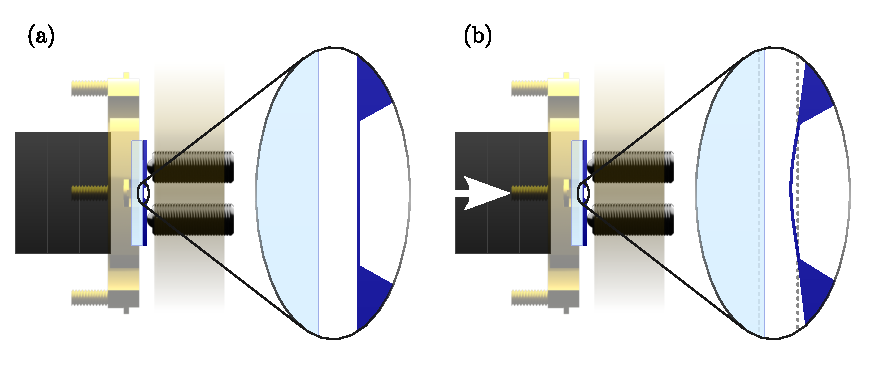
\includegraphics[width=\textwidth]{./chap5/fig/flexure tune.pdf}
    \caption{Cavity design and assembly. (a) In this configuration (no voltage applied to the piezos), the screws are used to align the membrane plane with respect to the back mirror plane, ensuring a good parallelism between both planes. (b) Flexure tuning of the membrane position. When a voltage is aplied to the piezos, they push on the back of the assembly, forcing the silicon frame to bend, thus displacing the membrane with respect to the back mirror. The two dashed lines show the initial positions of the back mirror and the membrane. This push shortens the overall cavity length (i.e. increasing the overall system's frequency), as well as the relative distance between the mirror and the membrane (i.e. changing the optomechanical coupling). }
    \label{fig:flexure tune}
\end{figure}


\color{black}

\subsection{Experimental Setup}
The assembly is now to be integrated into the optical setup shown in Fig.~\ref{fig:optical layout}. The source laser is a 1064nm Nd:YAG laser (Coherent Mephisto). We did not require the full optical power delivered by the laser, so a short optical path not detailed here splits the laser in 3 arms to eventually fiber couple some laser power and bring it to other experiments that would need 1064nm laser light. \newline

\begin{figure}[h!]
    \centering  
    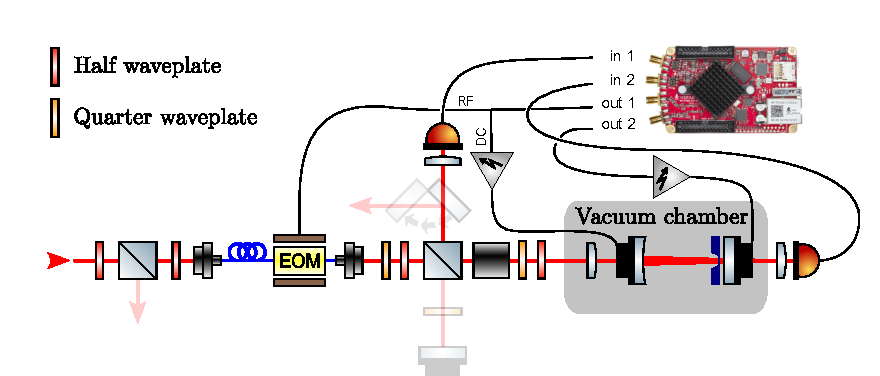
\includegraphics[width=\textwidth]{./chap5/fig/fig_lock_MATE.pdf}
    \caption{}
    \label{fig:optical layout}
\end{figure}
The optical path then consists of : 
\begin{itemize}
  \item a first half waveplate and a beam splitter to adjust the total power injected into the experimental setup,
  \item a fibered electro-optics phase modulator (EOM Photline NIR-MPX-LN-10) to generate sidebands for the PDH locking of the cavity. It is polarization matched by using a fibered polarization controller to avoid Residual Amplitude Modulation noise (RAM) at the output (three blue circles on the optical layout). 
  \item a fiber coupler to go from a guided optical mode to a free space optical mode, with a the coupler adjusted such that the outputted beam is collimated and has a waist of about 1mm,
  \item a quarter waveplate to compensate for ellipticity of the output beam polarization, then a half waveplate and a beam splitter to adjust the powers injected into the cavity path and the prospective LO path, respectively,
  \item on the cavity path, a faraday rotator to ensure the cavity reflected beam to be deflected to an output port and not back into the fiber 
  \item a lens to mode match the laser input mode to the cavity mode, with a focal length of 40 to 60mm depending on the input mirror radii of curvature. This lens is mounted on a x-y cage system translation mount, and is mounted inside the vacuum chamber that features AR coated windows to allow for optical access yet minimal parasite reflections.
  \item the cavity itself. 
  \item two photodiodes (Thorlabs ???) to detect the reflected beam and the transmitted beam, respectively, with 40mm focal length lenses to focus the beam onto the photodiodes. 
\end{itemize}

The optical path was designed to be as modular as possible, allowing for easy replacement of the components if needed, as well as additions of optical elements. For this reason, it features two fainted additional optical paths as seen on Fig.~\ref{fig:optical layout}, one for a prospective LO, and another to deflect the reflected beam to a Homodyne Detection setup using a flip mirror. Polarization optics would aslo need to be added on the Homodyne Detection path to mix the LO and the reflected beam, but this was not done during this thesis.

\subsection{Alignment Procedures}
The optical setup is now to be aligned as to ensure a good mode matching between the laser input mode and the cavity mode. The steps are as follows, and the associated diagrams are shown in Fig.~\ref{fig:tilt}:
\begin{itemize}
  \item \textbf{Step 1} (Fig.~\ref{fig:tilt}(a))\textbf{:} we position an iris diaphragm before our two injection mirrors mounted on ($\theta_x$,$\theta_y$) kinematic mounts. We then adjust the tilt of both mirrors i.e. \textit{beam-walking}, such that the reflected beam is centered on the iris diaphragm: this is done by maximising the reflected signal on the reflection photodiode. This ensure the beam reflected by the output mirror (HR mirror) is at normal incidence. In a second time we tune the plane of the resonator using the three screws of the assembly. We monitor the Fizeau fringes in transmission with a camera (Allied Vision Alvium), and adjust the tilt such that no fringes are to be seen. 
  \item \textbf{Step 2} (Fig.~\ref{fig:tilt}(b))\textbf{:} we then place the focusing lens in the optical path, and adjust its position such that we recover maximal power on the reflection photodiode. This lens is mounted on the (x-y) cage system translation mount, and positioned at a distance from the back mirror fixed by the cavity mode matching requirements (ref chap theory). The lens is then fixed in place using the cage system screws.
  \item \textbf{Step 3} (Fig.~\ref{fig:tilt}(c))\textbf{:} we add the input mirror on a ($\theta_x$,$\theta_y$) cage system mount, and adjust its position to get an input beam normal to the tangent of the concave mirror curvature. This is also done maximising the reflected power on the reflection photodiode. The mount (and thus the mirror) was also positioned at the appropriate distance from the back mirror to ensure optimal mode matching. 
  \item \textbf{Step 4} (Fig.~\ref{fig:tilt}(d))\textbf{:} We scan the cavity length using the piezo actuator mounted on the input mirror, and monitor the cavity resonances using both the reflected and transmitted photodiodes. We finally fine tune the mode match by \textit{beam-walking} the two injection mirrors. We can also play with the collimating lens at the fiber coupler (not shown on the diagram) as to fine tune for longitudinal mode matching. The cavity is now aligned and ready for operation.
  \end{itemize}

\begin{figure}[h!]
    \centering  
    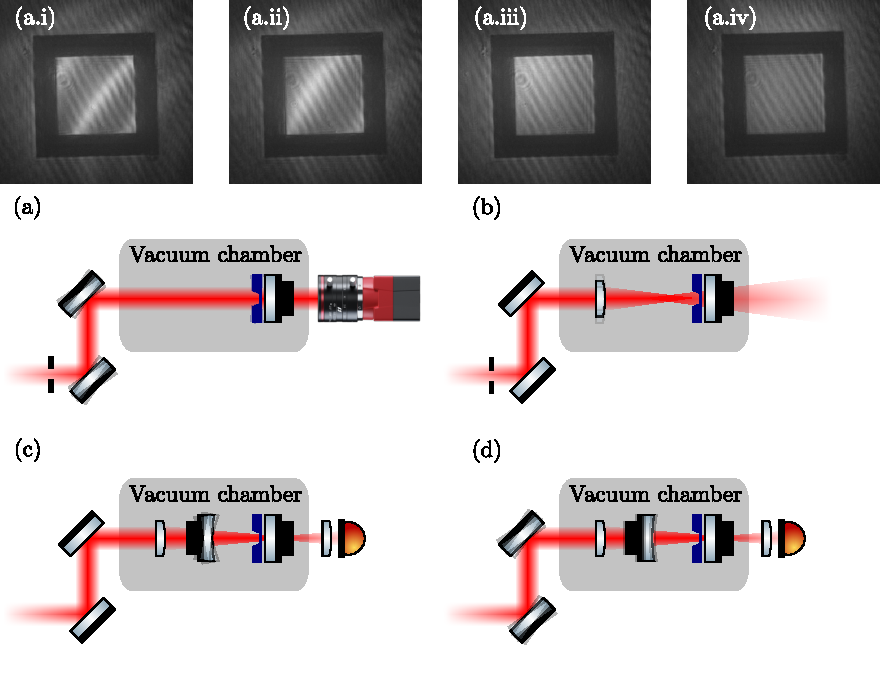
\includegraphics[width=\textwidth]{./chap5/fig/tilt_alignementB.pdf}
    \caption{Set up alignment procedure. (a) to (d) show the steps to align the cavity with respect to the optical path (detailed in the main text). The (a.i) to (a.iv) show what is seen on the camera 4 four different tilt positions where (a.iv) displays a 'good' tilt alignement: no visible fringes except for the dim fringes of the camera setup. These dim fringes are present when the beam is a normal incidence with the back mirror (use of the iris) and are believed to be intereferences arising from reflections inside the camera objective as they are seen whatever the plane of focus is. }
    \label{fig:tilt}
\end{figure}
\section{Experimental Characterization}
\subsection{Cavity Characterization}
Once the cavity is aligned, we can scan the cavity length by driving the front mirror piezo with a triangular or a sine wave voltage. This signal is first amplified using a high voltage amplifier made by the LKB electronic workshop, which can deliver up to 1000V. The output impedance of the amplifier is a standard 50 Ohms, but the piezo in derivation at the end of the line with capacitance of about 15 nF low pass filters the signal at  $\sim$ 200 Hz. We can also modulated the back piezo actuators, in DC or AC, and a similar lowpass filtering occurs with a lower cutoff frequency $\sim$ 50Hz (3 piezo actuators in parallel with a capacitance of around 100 nF each). We call the input mirror piezo voltage $V_{\text{SW}}$ as it is used to scan the cavity length, and the back piezo voltage $V_{\text{DC}}$ as it is used to set the membrane position, and we model the these voltages as third order polynomials of the actual displacements $L-x$ and $x$ respectively. \\

We then monitor the cavity resonances using both the reflected and transmitted photodiodes and scanning the cavity over a large range, as to mode match the cavity to the TEM00 mode. By beam walking, we optimally mode match the cavity such that higher order modes vanish in the photodiode noise floor and the reflected and transmitted signals are maximised, we can then perform finer scans to characterize the cavity parameters.

Using the IR EOM as a frequency ruler, setting a reference between few MHz to $\sim$ 60 MHz (limited by the RedPitaya) we perform lorentzian fits of the three lorentzian dips, and compare the fitted positions. Two typical scans are shown in Fig.~\ref{fig:cavity_scan}, one large scan over few cavity FSRs, and a narrow one. \\ 

\noindent  \textbf{Finesse :} We can used three different methods to evalutate the finesse of the cavity. 
\begin{itemize}
  \item The first one would be to scan the cavity over few FSRs, and fit the lorentzian dips such that we can extract the ratio of their interspacings to their linewidths. This method is quite sensitive to the piezo nonlinearities, arising both from the system's transfer function and from the low pass filtering of the voltage ramp by the electronics. One can however used a sine ramp below the electronics cutoff frequency and calibrate the disaplcement owing to the fact that each resonance corresponds to a displacement of $\lambda/2$ (one FSR). 
  \item The second method would be to scan the cavity over a single resonance, and use the EOM sidebands as a frequency reference to extract the linewidth of the resonance. This method is less sensitive to piezo nonlinearities, assuming the piezo sweep is quasi linear over the resonance width. 
  \item The third method would be to scan the cavity rapidly and observe a cavity ringdown, and compare the heights of the first two rebounds in transmission to their temporal spacings. This method is less sensitive to piezo nonlinearities, but requires a fast photodiode. Additionally we can vary the piezo sweep frequency to scan for various sweep rates. 
\end{itemize}

Many trial and errors for such a MATE cavity were realised over this thesis, but the cleaner data were obtained with a cavity made of an input concave mirror of radius of curvature $R=20mm$ and transmittivity $t_1=100ppm$, a plane back mirror of $t_2=20ppm$ and a cavity length of $L=17mm$. Hence, the theoretical finesse would be $\sim 52400$. \\ 

\noindent \textbf{Empty cavity: }By using the second method for our finesse estimation, the empty cavity finesse was measured to be $\sim 28000$, such that we deduce total loss of $\Sigma T_i = 225 \pm 20$ppm  (including losses). The LMA did not provide us with specification sheets for the exact mirrors we used, but the uncertainty on the sum of the transmissions is estimated to be around 15ppm. In turn, we can estimate the excess cavity losses to be around $\gamma = 105ppm$. \color{red} errors \color{black} \\

\noindent \textbf{MATE cavity: }Once the membrane is inserted inside the cavity, both the resonant frequencies and the linewidths-finesse vary as a function of the membrane position $x$. Using our third order polynomials to model the piezos voltage seed to displacements transduction, we renormalize both the input mirror voltage sweep $V_{\text{SW}}$ and the back mirror voltage DC $V_{\text{DC}}$ to the cavity FSR and the nominal membrane displacement $x$ respectively. Knowing or laser wavelenth, this fit allows us to estimate the membrane reflectivity $|r_m|$ which is found to be 0.54. \color{red} link to expected value \color{black} \\ 

These fits then give us the total maps of available displacements $L-x$ and $x$ as a function of both $V_{\text{SW}}$ and $V_{\text{DC}}$, as shown in Fig.~\ref{fig:maps}. \\ 

\begin{figure}[h!]
    \centering  
    \includegraphics[width=\textwidth]{./chap5/fig/scansTot.pdf}
    \caption{ }
    \label{fig:tilt}
\end{figure}

\begin{figure}[h!]
    \centering  
    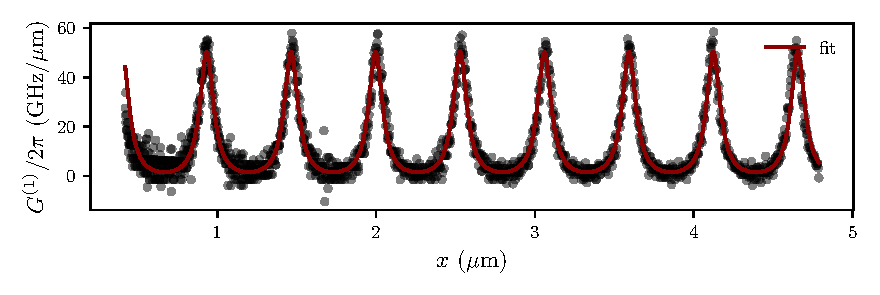
\includegraphics[width=\textwidth]{./chap5/fig/scancoupling.pdf}
    \caption{ }
    \label{fig:tilt}
\end{figure}

\begin{figure}[h!]
    \centering  
    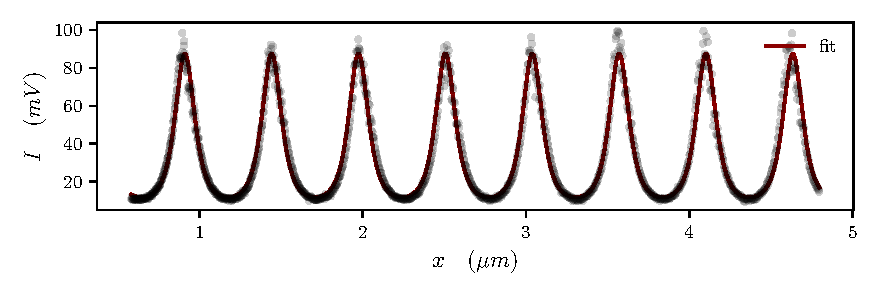
\includegraphics[width=\textwidth]{./chap5/fig/scantrans.pdf}
    \caption{ }
    \label{fig:tilt}
\end{figure}

\noindent \textbf{Position dependent finesse: } We now record cavity scans at increasing values of $V_{DC}\propto P_3(x)$. The finesse oscillates between $\sim 6000$ and $\sim 20000$, which corresponds to total losses $\Sigma T_i$ between 300ppm and 1050ppm. This is significantly higher than the empty cavity losses, which indicates that the membrane introduces significant additional losses. 

Using the IR EOM as a frequency ruler, we can perform slow scans of the cavity length while monitoring the transmitted intensity. By carefully controlling the piezo voltage and using a lock-in amplifier to extract the signal, we can obtain high-resolution measurements of the cavity resonances. This technique allows us to probe the cavity modes with great precision and is particularly useful for characterizing the effects of the membrane on the cavity dynamics.
\subsection{Locking Techniques and Stability}
\subsection{Optical Ringdowns and Loss Measurements}
\subsection{Mechanical Resonator Characterization}
\subsection{Bistability}

\section{Design of an Optomechanical Fibered Cavity}
\subsection{Design considerations}

\vspace{-\baselineskip}



\chapter{Experiments: \\ Frequency Dependent Squeezing}
This chapter will cover the experimental methods used in the development of frequency-dependent squeezing in optomechanical systems, focusing on the generation of squeezed light, optical locking techniques, and quadrature measurement methods. The methods are designed to enhance the sensitivity of measurements in quantum optics and optomechanics.
\minitoc
\newpage 

\section{OPO Resonance and Locking}
\subsection{Resonance Conditions and Sweeps}
\subsection{Lock Acquisition and Optimization}
\subsection{Stability Characterization}
\section{Quadrature Spectral Analysis}
\subsection{Detection of Squeezing and Anti-squeezing}
\subsection{Spectral Variation with Frequency}
\subsection{Optimal Quadrature Conditions}
\section{Filter Cavity Concept}
\subsection{Virgo Filter Cavity }
\subsection{Thermal effects in bichromatic locks}

\appendix
% !TeX encoding = UTF-8
% !TeX spellcheck = fr_FR
% !TeX root = mythesis.tex

\chapter*{Appendix 1: Derivation of the PDH Error Signal }\label{app:PDH}
\addcontentsline{toc}{section}{Appendix: PDH Derivation}

In this appendix, we derive the Pound-Drever-Hall (PDH) error signal starting from the real, quantum-normalized phase-modulated electric field expression. We aim to show how the demodulated signal is a linear combination of the real and imaginary parts of the cavity reflection coefficient, with the demodulation phase selecting the appropriate quadrature for locking.

\subsection*{1. Input Phase-Modulated Field}

The electric field at the input of the cavity is assumed to be a coherent state that has been phase-modulated at frequency \( \Omega \), such that the classical (real) electric field takes the form:
\begin{equation}
    E_{\text{cl}}^{(\text{PM})}(t) = i \sqrt{\frac{\hbar \omega_0}{2 \varepsilon_0}} \, \alpha_0 \left[
        e^{-i\omega_0 t} - e^{i\omega_0 t}
        + \frac{i \epsilon_\phi}{2} \left( e^{-i(\omega_0 - \Omega)t} + e^{i(\omega_0 - \Omega)t} \right)
        + \frac{i \epsilon_\phi}{2} \left( e^{-i(\omega_0 + \Omega)t} + e^{i(\omega_0 + \Omega)t} \right)
    \right]
    \label{eq:pm_field}
\end{equation}
where \( \alpha_0 \) is the coherent amplitude of the carrier, \( \epsilon_\phi \ll 1 \) is a small modulation index (related to the phase modulation depth), and \( \omega_0 \) is the optical carrier frequency. This field includes both the positive and negative frequency components, as expected for a physical (Hermitian) electric field operator.

\subsection*{2. Reflection from the Cavity}

Each frequency component of the field is reflected with a complex frequency-dependent amplitude reflection coefficient \( r(\omega) \), such that the reflected field is:
\begin{equation}
\begin{aligned}
    E_{\text{refl}}(t) = i \sqrt{\frac{\hbar \omega_0}{2 \varepsilon_0}} \, \alpha_0 \Big[
    & r(\omega_0) e^{-i\omega_0 t} - r^*(\omega_0) e^{i\omega_0 t} \\
    & + \frac{i \epsilon_\phi}{2} \left( r(\omega_0 - \Omega) e^{-i(\omega_0 - \Omega)t} + r^*(\omega_0 - \Omega) e^{i(\omega_0 - \Omega)t} \right) \\
    & + \frac{i \epsilon_\phi}{2} \left( r(\omega_0 + \Omega) e^{-i(\omega_0 + \Omega)t} + r^*(\omega_0 + \Omega) e^{i(\omega_0 + \Omega)t} \right)
    \Big]
\end{aligned}
\label{eq:refl_field}
\end{equation}

\subsection*{3. Photodetected Intensity}

The photodetector measures the intensity:
\[
I(t) \propto |E_{\text{refl}}(t)|^2
\]
We isolate the terms oscillating at \( \Omega \), which arise from the interference between the carrier and sideband components. Keeping only the beat terms between the carrier and sidebands, we find:
\begin{equation}
I(t) \supset \epsilon_\phi \cdot \Re\left[ A_+ - A_- \right] \cos(\Omega t)
+ \epsilon_\phi \cdot \Im\left[ A_+ - A_- \right] \sin(\Omega t)
\label{eq:intensity_beats}
\end{equation}
where we define:
\[
A_\pm = r(\omega_0) r^*(\omega_0 \pm \Omega)
\]

\subsection*{4. Demodulation with Arbitrary Phase}

The signal is demodulated using a local oscillator \( \cos(\Omega t + \phi) \), where \( \phi \) is the demodulation phase. Using trigonometric identities:
\[
\cos(\Omega t + \phi) = \cos(\Omega t)\cos\phi - \sin(\Omega t)\sin\phi
\]
we multiply Equation~\eqref{eq:intensity_beats} and low-pass filter to obtain:
\begin{equation}
\epsilon_{\text{PDH}}(\phi) \propto \epsilon_\phi \left\{
\Re[A_+ - A_-] \cos\phi + \Im[A_+ - A_-] \sin\phi
\right\}
\label{eq:error_signal_general}
\end{equation}

\subsection*{5. Sidebands Far Off-Resonance Approximation}

In the standard PDH regime, the modulation frequency is much greater than the cavity linewidth:
\[
\Omega \gg \kappa
\]
so the sidebands are far off-resonance. This means:
\[
r(\omega_0 \pm \Omega) \approx 1 \quad \Rightarrow \quad A_\pm \approx r(\omega_0)
\]
and therefore:
\[
A_+ - A_- \approx 0
\]
However, if we retain the asymmetry between the sidebands (e.g., due to dispersion), or keep the finite detuning contribution, we approximate:
\[
A_+ - A_- \approx r(\omega_0) \left[ r^*(\omega_0 + \Omega) - r^*(\omega_0 - \Omega) \right] = r(\omega_0) \Delta r^*
\]

\subsection*{6. Final Result}

Substituting into Equation~\eqref{eq:error_signal_general}, we obtain:
\begin{equation}
\epsilon_{\text{PDH}}(\phi) \propto \epsilon_\phi \left\{
\Re[r(\omega_0) \Delta r^*] \cos\phi + \Im[r(\omega_0) \Delta r^*] \sin\phi
\right\}
\label{eq:error_signal_deltar}
\end{equation}

In the limit where \( \Delta r^* \rightarrow 1 \) (normalized, symmetric sidebands), this simplifies to:
\begin{equation}
\boxed{
\epsilon_{\text{PDH}}(\omega_0, \phi) \propto \cos\phi \cdot \Re[r(\omega_0)] + \sin\phi \cdot \Im[r(\omega_0)]
}
\label{eq:pdh_final}
\end{equation}

\subsection*{7. Interpretation}

Equation~\eqref{eq:pdh_final} shows that the demodulated error signal is a linear superposition of the real and imaginary parts of the complex reflection coefficient. The demodulation phase \( \phi \) selects the detected quadrature:
\begin{itemize}
    \item \( \phi = 0 \): error signal is proportional to \( \Re[r] \) — symmetric around resonance, not suitable for locking.
    \item \( \phi = \pi/2 \): error signal is proportional to \( \Im[r] \) — antisymmetric, ideal dispersive error signal.
    \item \( \phi \ne 0, \pi/2 \): mixes quadratures, possibly introducing offset or distortion.
\end{itemize}

\bigskip

This derivation makes explicit how the PDH method uses phase-sensitive detection to extract the component of the reflection coefficient that varies linearly with detuning, enabling precise feedback locking of the laser to the cavity resonance.

\chapter*{Appendix 2: Spectra derivation  }\label{app:spectra}
\addcontentsline{toc}{section}{Appendix: Spectra Derivation}

\begin{align}
\hat p[\Omega]
&= 2\,|\alpha| \Big( \delta[\Omega] + \Re\{\varepsilon[\Omega]\} \Big)
  + \delta \hat p[\Omega] \,,
\\[4pt]
\hat p[\Omega]\;\hat p[\Omega']
&= 4|\alpha|^{2}\Big(
      \delta[\Omega]S[\Omega']
    + \delta[\Omega]\Re\{\varepsilon[\Omega']\}
    + \delta[\Omega']\Re\{\varepsilon[\Omega]\}
    + \Re\{\varepsilon[\Omega]\}\Re\{\varepsilon[\Omega']\}
  \Big)
  + \delta \hat p[\Omega]\;\delta \hat p[\Omega'] \,,
\\[6pt]
\big\langle \cdots \big\rangle
&= 4|\alpha|^{2}\Big(
      \delta(\Omega)\,\delta(\Omega')
    + \frac{\varepsilon}{2}\,\delta(\Omega)\,\delta(\Omega'-\Omega_m)
    + \frac{\varepsilon}{2}\,\delta(\Omega)\,\delta(\Omega'+\Omega_m)
\\[-2pt]&\hphantom{= 4|\alpha|^{2}\Big(}
    + \frac{\varepsilon}{2}\,\delta(\Omega')\,\delta(\Omega-\Omega_m)
    + \frac{\varepsilon}{2}\,\delta(\Omega')\,\delta(\Omega+\Omega_m)
\\[-2pt]&\hphantom{= 4|\alpha|^{2}\Big(}
    + \frac{\varepsilon^{2}}{4}\Big[
          \delta(\Omega-\Omega_m)\,\delta(\Omega'+\Omega_m)
        + \delta(\Omega-\Omega_m)\,\delta(\Omega'-\Omega_m)
\\[-2pt]&\hphantom{= 4|\alpha|^{2}\Big(+ \frac{\varepsilon^{2}}{4}\Big[}
        + \delta(\Omega+\Omega_m)\,\delta(\Omega'+\Omega_m)
        + \delta(\Omega+\Omega_m)\,\delta(\Omega'-\Omega_m)
      \Big]
  \Big)
  + \big\langle \delta p[\Omega]\;\delta p[\Omega'] \big\rangle \,.
\end{align}





\chapter*{Derivation of the optimal angle}
\subsection*{Optimal fixed homodyne angle with complex \texorpdfstring{$\mathcal{K}$}{K}}

Assume the measured (reflected) quadrature is
\[
\delta q_r \;=\; \delta q_{\rm in} \;+\; \mathcal{K}\,\delta p_{\rm in},
\]
so that, for any input covariance matrix \(S^{\rm in}\),
\[
S^{r}_{qq} \;=\; S^{\rm in}_{qq} + |\mathcal{K}|^{2}S^{\rm in}_{pp} + 2\,\mathrm{Re}\{\mathcal{K}\}\,S^{\rm in}_{pq}.
\]

For an input squeezed state of strength \(R\) and angle \(\theta\),
\[
S^{\rm in}(r,\theta)=
\begin{pmatrix}
\cosh 2r + \sinh 2r \cos 2\theta & \,-\sinh 2r \sin 2\theta\\[2pt]
\,-\sinh 2r \sin 2\theta & \cosh 2r - \sinh 2r \cos 2\theta
\end{pmatrix}.
\]
Hence
\begin{align}
S^{r}_{qq}(\theta)
&= \cosh 2r - \sinh 2r \cos 2\theta
 + |\mathcal{K}|^{2}\!\left(\cosh 2r + \sinh 2r \cos 2\theta\right)
 - 2\,\mathrm{Re}\{\mathcal{K}\}\,\sinh 2r \sin 2\theta \nonumber\\[2pt]
&= (1+|\mathcal{K}|^{2})\cosh 2r
  - (1-|\mathcal{K}|^{2})\sinh 2r \cos 2\theta
  - 2\,\mathrm{Re}\{\mathcal{K}\}\,\sinh 2r \sin 2\theta .
\label{eq:Sqq_linearform}
\end{align}

\paragraph{Optimal fixed angle.}
Differentiate \eqref{eq:Sqq_linearform} w.r.t.~\(\theta\) and set to zero:
\[
\frac{\partial S^{r}_{qq}}{\partial \theta}
= 2\sinh 2r\Big[(1-|\mathcal{K}|^{2})\sin 2\theta - 2\,\mathrm{Re}\{\mathcal{K}\}\cos 2\theta\Big]=0,
\]
which gives the optimal fixed readout angle
\begin{equation}
\tan(2\theta_{\rm opt})
=  \frac{2\,\mathrm{Re}\{\mathcal{K}\}}{\,1-|\mathcal{K}|^{2}\,}
\qquad
\label{eq:theta_opt}
\end{equation}
Writing \(\mathcal{K}=|\mathcal{K}|e^{i\varphi_m}\) one may also use
\[
\tan(2\theta_{\rm opt})=\frac{2|\mathcal{K}|\cos\varphi_m}{\,1-|\mathcal{K}|^{2}\,}.
\]

\paragraph{Minimum attained value.}
Plugging the optimal angle back into \eqref{eq:Sqq_linearform} then yields
\begin{equation}
\quad
S^{r}_{qq,\min}
=(1+|\mathcal{K}|^{2})\cosh 2r - \sqrt{(1-|\mathcal{K}|^{2})^{2}+\big(2\,\mathrm{Re}\{\mathcal{K}\}\big)^{2}}\,\sinh 2r,
\label{eq:Smin_general}
\end{equation}

\paragraph{Lower bound and the real-\(\mathcal{K}\) case.}
In the free mass limit, \(\mathcal{K}\) is purely real, so that \(\varphi_m=0\) and \(\mathrm{Re}\{\mathcal{K}\}=|\mathcal{K}|\). In this case, the minimum variance \eqref{eq:Smin_general} reduces to
\[
S^{r}_{qq,\min}=(1+|\mathcal{K}|^{2})e^{-2r} 
\]
%%%%%%%%%%%%%%%%%%%%%%%%%%%%%% FINAL PAGES %%%%%%%%%%%%%%%%%%%%%%%%%%%%%%%%%%
\backmatter
%%%%%%%%%%%%%%%%%%%%%%%%%%%%  BIBLIOGRAPHY %%%%%%%%%%%%%%%%%%%%%%%%%%%%%%%%%%
\cleardoublepage
\phantomsection
% \addcontentsline{toc}{chapter}{Bibliographie}
%%%%% use of BiBTeX:
% \bibliographystyle{these/bib/thesefr-href}
% \bibliography{these/bib/references_these.bib}
%%%%% to be replaced by,  for final version:
%\intput{mythesis.bbl}
%%%%%%%%%%%%%%%%%%%%%%%%%  4th COVER %%%%%%%%%%%%%%%%%%%%%%%%%%%%%%%%%%%%%%%%
\backcover % requires thcover.sty loaded and thcoverdata.tex filled
\end{document}